% updated April 2002 by Antje Endemann
% Based on CVPR 07 and LNCS, with modifications by DAF, AZ and elle, 2008 and AA, 2010, and CC, 2011; TT, 2014; AAS, 2016; AAS, 2020

\documentclass[runningheads]{llncs}
\usepackage{graphicx}
\usepackage{comment}
\usepackage{amsmath,amssymb} % define this before the line numbering.
\usepackage{color}

% INITIAL SUBMISSION - The following two lines are NOT commented
% CAMERA READY - Comment OUT the following two lines
\usepackage{ruler}
\usepackage[width=122mm,left=12mm,paperwidth=146mm,height=193mm,top=12mm,paperheight=217mm]{geometry}

\DeclareMathOperator*{\argmax}{arg\,max}
\DeclareMathOperator*{\argmin}{arg\,min}
\usepackage{mathrsfs}
\newcommand{\RED}[1]{#1}

% \newcommand\TODO[1]{{\color{red}{TODO: #1}}}
\newcommand\TODO[1]{#1}
% \newcommand\UPDATE[1]{{\color{blue}{#1}}}
\newcommand\UPDATE[1]{#1}
\newcommand\SOURCE[1]{{\color{green}{(from: #1)}}}
\newcommand*{\maskname}{central instance~}
\newcommand*{\sparseBr}{sparse-neighborhood~}
\newcommand*{\denseBr}{dense-neighborhood~}
\newcommand*{\encBr}{encoded-neighborhood~}
\newcommand*{\maskDec}{central-mask-decoder~}
\newcommand*{\evidW}{w}
\usepackage[e]{esvect}
\usepackage{bm}
\usepackage{pifont}
\newcommand{\cmark}{\ding{51}}%
\newcommand{\xmark}{\ding{55}}%

% \newcommand\coord{\vec}
\newcommand\coord{\bm}

\usepackage{tabularx}
\usepackage{multirow}
\usepackage{makecell}
\usepackage{textcomp}
\usepackage{booktabs}
% \usepackage[labelformat=simple]{subcaption}
\newcolumntype{M}[1]{>{\centering\arraybackslash}m{#1}}
\newcolumntype{R}[1]{>{\raggedleft\arraybackslash}m{#1}} 
\newcolumntype{L}[1]{>{\raggedright\arraybackslash}m{#1}} 
\newcolumntype{?}{!{\vrule width 0.3em}}

\usepackage{algorithm}% http://ctan.org/pkg/algorithm
\PassOptionsToPackage{noend}{algpseudocode}% comment out if want end's to show
\usepackage{algpseudocode}% http://ctan.org/pkg/algorithmicx
\algrenewcommand\algorithmicindent{0.8em}

\makeatletter
\newcommand*{\skipnumber}[2][1]{%
   {\renewcommand*{\alglinenumber}[1]{}\State #2}%
   \addtocounter{ALG@line}{-#1}}
\renewcommand{\ALG@beginalgorithmic}{\small}
\makeatother

\usepackage[dvipsnames]{xcolor}
\usepackage{hyperref}

\begin{document}
% \renewcommand\thelinenumber{\color[rgb]{0.2,0.5,0.8}\normalfont\sffamily\scriptsize\arabic{linenumber}\color[rgb]{0,0,0}}
% \renewcommand\makeLineNumber {\hss\thelinenumber\ \hspace{6mm} \rlap{\hskip\textwidth\ \hspace{6.5mm}\thelinenumber}}
% \linenumbers
\pagestyle{headings}
\mainmatter
\def\ECCVSubNumber{4210}  % Insert your submission number here

\title{Proposal-free volumetric instance segmentation from latent single-instance masks} % Replace with your title

% INITIAL SUBMISSION 
%\begin{comment}
\titlerunning{ECCV-20 submission ID \ECCVSubNumber} 
\authorrunning{ECCV-20 submission ID \ECCVSubNumber} 
\author{Anonymous ECCV submission}
\institute{Paper ID \ECCVSubNumber}
%\end{comment}
%******************

% CAMERA READY SUBMISSION
\begin{comment}
\titlerunning{Abbreviated paper title}
% If the paper title is too long for the running head, you can set
% an abbreviated paper title here
%
\author{First Author\inst{1}\orcidID{0000-1111-2222-3333} \and
Second Author\inst{2,3}\orcidID{1111-2222-3333-4444} \and
Third Author\inst{3}\orcidID{2222--3333-4444-5555}}
%
\authorrunning{F. Author et al.}
% First names are abbreviated in the running head.
% If there are more than two authors, 'et al.' is used.
%
\institute{Princeton University, Princeton NJ 08544, USA \and
Springer Heidelberg, Tiergartenstr. 17, 69121 Heidelberg, Germany
\email{lncs@springer.com}\\
\url{http://www.springer.com/gp/computer-science/lncs} \and
ABC Institute, Rupert-Karls-University Heidelberg, Heidelberg, Germany\\
\email{\{abc,lncs\}@uni-heidelberg.de}}
\end{comment}
%******************
\maketitle


% !TEX root = ../patchEmbeddings_review.tex

\begin{abstract}
The abstract should summarize the contents of the paper. LNCS guidelines
indicate it should be at least 70 and at most 150 words. It should be set in 9-point
font size and should be inset 1.0~cm from the right and left margins.
\dots
\keywords{We would like to encourage you to list your keywords within
the abstract section}
\end{abstract}


% !TEX root = ../patchEmbeddings_review.tex

\section{Introduction}\label{sec:intro}

\emph{Instance segmentation} is a task of computer vision consisting in assigning each pixel of an image to an object instance. %, where the number of instances is usually not known in advance. 
% The most success in instance segmentation (IS) has been achieved by applying deep learning. %\cite{he2017mask,romera2016recurrent,liu2018affinity}. 
There are two main types of successful deep learning approaches to instance segmentation: proposal-based and proposal-free methods. 
Proposal-based methods consist of two steps: object detection, for example by finding bounding boxes, and assigning pixels to the detected objects. These approaches have proven to be highly successful in instance segmentation competitions like MS COCO \cite{lin2014microsoft} and CityScapes \cite{cordts2016cityscapes}. 
On the other hand, proposal-free methods adopt a bottom-up approach by directly grouping pixels into instances. Recently, there has been a growing interest for such methods that do not involve object detection, since, in certain types of images like the ones we focus on in this work, object instances cannot be approximated by bounding boxes and are usually larger than the field of view of the model.  

 
% A graph partitioning algorithm is used to obtain object instances.
Some recent successful proposal-free approaches \cite{januszewski2018high,meirovitch2016multi,liu2016multi} tackle instance segmentation by predicting, for a given patch of the input image, whether or not each pixel in the patch is part of the same instance associated to the central/anchor pixel. 
These masks are then repeatedly predicted, in a sliding window style, across the entire image and 
the final object-instances are obtained by aggregating predictions from overlapping masks.
In the following, we will refer to these patch predictions as \emph{\maskname masks}.

In this work, we propose a novel proposal-free segmentation method that is also based on the prediction of \maskname masks. However, our approach comes with the following four main advantages.
Firstly, our model concurrently predicts all \maskname masks, one for each pixel, by using a fully-convolutional approach and comes then with a much lower computational cost compared to previous patch-based methods iteratively predicting one instance at the time, one mask after the other \cite{januszewski2018high,meirovitch2016multi}.
Secondly, our approach predicts \maskname masks in a low dimensional latent representation, which allows great memory savings and let us apply the method to large volumetric images of neuron tissue \cite{arganda2015crowdsourcing}. 
Thirdly, the proposed approach aggregates predictions from overlapping \maskname masks without the need of any extra parameter or threshold;
and, finally, all final object-instances are obtained concurrently, as opposed to previous methods predicting them one-by-one with subsequent conflict resolution. 
% by extracting a set of affinities that are then used as signed weights of a graph representing the image, so that each node corresponds to a pixel

% Despite the recent successful application of patch-based methods, so far no study has been conducted to compare them with 

We also carry out a systematic study to compare the proposed model with another really common proposal-free method that has been recently successfully applied both to natural \cite{liu2018affinity,Gao_2019_ICCV} and biological \cite{lee2017superhuman,wolf2018mutex,bailoni2019generalized} images. This alternative method is sketched in Fig. \ref{fig:main_figure}a and consists of a fully-convolutional network predicting, for each pixel, a small set of short- and long-range affinities, i.e. neighborhood relations representing how likely it is for a pair of pixels to belong to the same object instance. 
\TODO{} Our comparison on neuron segmentation shows how... (equally efficient, results, etc...)


% In this work, we focus on a proposal-free method, where a Convolutional Neural Network (CNN) is trained to predict, for every pixel $i$ in the image, a patch of fixed size representing a probability mask of the instance object to which pixel $i$ belongs. The mask predicted in each patch is centered at the corresponding pixel $i$ and represents then a dense local neighborhood structure of pixel $i$. Whenever the object instance associated to pixel $i$ is bigger than the size of the patch, only a partial probability mask of the object is predicted. 
% In the following, we will call these masks as \patch or LSPM.

% [A naive way to predict one $K\times K$ \patch  for each pixel in an image would be to use a fully convolutional model with $K^2$ output channels, where each channel represents a pixel of the corresponding mask. However, this approach would not scale up well with increasing sizes $K$.]

% Our first contribution is a fully convolutional model that predicts, for every pixel $i$, a representation of the associated $i$-th self-probability mask in a lower dimensional space (see Fig. \ref{fig:main_figure}). This is possible due to the fact that, among all possible neighborhood structures represented by local self-probability masks, only few of them are associated to occurring ground truth binary masks. Thus, the information included in the predicted self-probability masks can be easily encoded in a lower dimensional latent space. 



% As a second contribution, we propose two methods for converting the predicted per-pixel self-probability masks into edge weights of a graph representing the image, so that each node corresponds to a pixel and a graph clustering algorithm is used to obtain the final instance segmentation... \TODO{Parameter-free alg. to compute edge weights; experiments; summary of sections}
% One of the two methods results in a pipeline that is as efficient as the currently winning method of the CREMI challenge \emph{(more efficient actually, because of LMC...), but achieves better accuracies and, as our results shows, outputs more consistent neighborhood structures...}.
% The second proposed method yields a parameter-free algorithm achieving competitive performances, yada yada yada... 


\begin{figure}[t]
\centering
        % \includegraphics[width=0.4\textwidth,trim=0.25in 0.25in 0.68in 0.36in,clip]{./figs/SSBM_experiments.pdf} % 0.45
        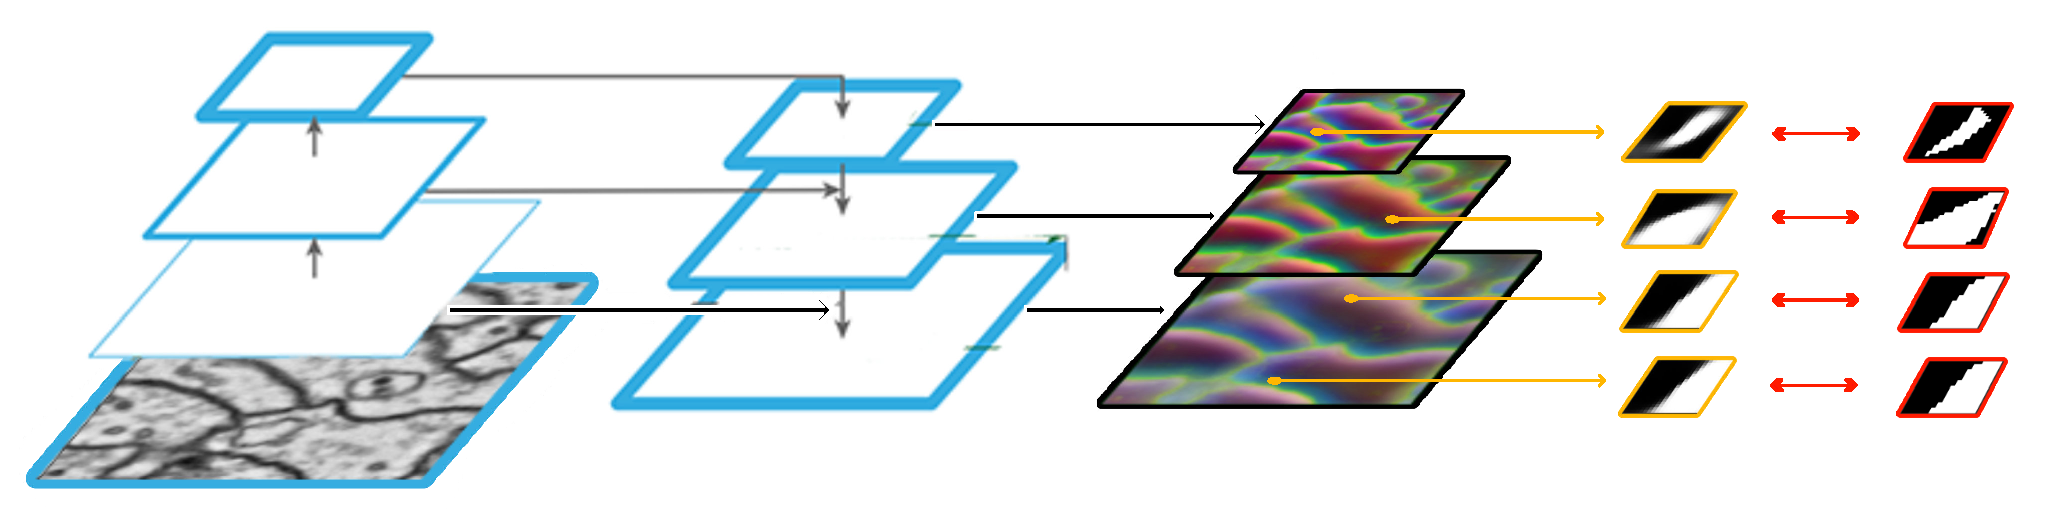
\includegraphics[width=\textwidth]{./figs/main_image.pdf} % 0.45
        \caption{A.) Predicting a sparse stencil of short- and long-range affinities. b) Predicting all patches (that it was actually the main proposal of PatchPerPix)...}
    \label{fig:main_figure}
\end{figure}




% !TEX root = ../patchEmbeddings_review.tex

\section{Related work} \label{sec:related_work}
\TODO{restructure, to be completed}

\textbf{Proposal-based methods} have been highly successful in instance segmentation competitions like MS COCO \cite{lin2014microsoft}, Pascal VOC2012 \cite{everingham2010pascal} and CityScapes \cite{cordts2016cityscapes}. They decompose the instance segmentation task into two steps that consists in generating object proposals and assigning to each bounding box a class and a binary segmentation mask \cite{he2017mask,porzi2019seamless,liu2018path,yang2012layered,li2017fully,ladicky2010and,hariharan2014simultaneous,chen2015multi,dai2016instance,liang2016reversible}. 
% They commonly rely on {Faster-RCNN}~\cite{ren2015faster} and can be trained end-to-end using non-maximum suppression. 
Other methods use instead recurrent models to sequentially generate instances one-by-one \cite{romera2016recurrent,ren2017end}.

\textbf{Proposal-free methods} adopt a bottom-up approach by directly grouping pixels into instances. Recently, there has been a growing interest for such  methods that do not involve object detection, since, in certain types of data, object instances cannot be approximated by bounding boxes. For example, the approach proposed in \cite{kirillov2017instancecut} uses a combinatorial framework for instance segmentation, 
% SGN \cite{liu2017sgn} sequentially group pixels into lines and then instances;
whereas a watershed transform is learned in \cite{bai2017deep} by also predicting its gradient direction. 
% whereas the template matching \cite{uhrig2016pixel} deploys scene depth information.
Others use metric learning to predict high-dimensional associative pixel embeddings that map pixels of the same instance close to each other, while mapping pixels belonging to different instances further apart \cite{lee2019learning,fathi2017semantic,newell2017associative,de2017semantic}. % kulikov2018instance
Final instances are then retrieved by applying a clustering algorithm, like in the end-to-end trainable mean-shift pipeline of \cite{kong2018recurrentPix}. 
Other recent successful methods simply let the model predict the relative coordinates of the instance center \cite{neven2019instance,cheng2019panopticdeeplab} or, given a point $(x,y)$ in the image, they train a model to generate the mask of the instance located at $(x,y)$ \cite{sofiiuk2019adaptis}. 

\textbf{Edge detection} also experienced recent progress thanks to deep learning, both on natural images \cite{Gao_2019_ICCV,liu2018affinity,xie2015holistically,kokkinos2015pushing} and biological data \cite{lee2017superhuman,schmidt2018cell,meirovitch2016multi,ciresan2012deep}. In neuron segmentation for connectomics, a field of neuroscience we also address in our experiments, boundaries are converted to final instances with subsequent postprocessing and superpixel-merging:
some use loopy graphs \cite{kaynig2015large,krasowski2015improving} or trees \cite{meirovitch2016multi,liu2016sshmt,liu2014modular,funke2015learning,uzunbas2016efficient} to represent the region merging hierarchy; the lifted multicut \cite{beier2017multicut} formulates the problem in a combinatorial framework, whereas 
flood-filling networks \cite{januszewski2018high} and MaskExtend \cite{meirovitch2016multi} use a CNN to iteratively grow one region/neuron at the time; recently, the work of \cite{meirovitch2019cross} made the process more efficient by employing a combinatorial encoding of the segmentation.
A structured learning approach was also proposed in \cite{funke2018large,turaga2009maximin}.

\TODO{}
 average linkage \cite{liu2018affinity,lee2017superhuman}, linkage learned by a random forest classifier \cite{nunez2013machine,knowles2016rhoananet}.


Extra approaches based signed graphs: Modern integer linear programming solvers can tackle problems of considerable size \cite{andres2012globally}, but accurate approximations \cite{pape2017solving,beier2016efficient,yarkony2012fast}, greedy agglomerative algorithms \cite{levinkov2017comparative,wolf2019mutex,keuper2015efficient,kardoostsolving} and persistence criteria \cite{lange2018partial,lange2018combinatorial} have been proposed for even larger graphs. 


proposal-free methods \cite{liu2018affinity,wolf2018mutex,lee2017superhuman} to predict long-range relationships between pixels.

\TODO{} patchPerPix, embeddings on connectomics


% !TEX root = ../patchEmbeddings_review.tex

\section{Model and training strategy}\label{sec:model}
In this section, we first define \maskname masks and briefly review a common strategy to train affinities for a sparse neighborhood.
Then, in Sec. \ref{sec:encoding_masks}, we present our first main contribution, i.e. a model trained end-to-end to predict encoded \maskname mask, one for each pixel of the input image. 
% Finally, in Sec. \ref{sec:multiscale_patches}, we show how we predicted \maskname masks at different scales.

\subsection{Local \maskname masks}\label{sec:self_masks}
This work proposes to distinguish between different object instances based on instance-aware pixel-pair affinities, which specifies whether two pixels belong to the same instance or not.
Given a pixel of the input image with coordinates $\coord{u}= (u_x, u_y)$, then a set of affinities to neighboring pixels within a $K\times K$ window is learned, where $K$ is an odd number. 
We define the $K\times K$-neighborhood of a pixel as:
\begin{equation}
\mathcal{N}_{K\times K} \equiv \mathcal{N}_{K} \times \mathcal{N}_{K}, \qquad \text{where} \quad \mathcal{N}_{K} \equiv \left\{-\frac{K-1}{2}, \ldots, \frac{K-1}{2}\right\}
\end{equation}
and represent the affinities associated to pixel $\coord{u}$ as a \maskname mask, i.e. a function $\mathcal{M}_{\coord{u}}: \mathcal{N}_{K\times K} \rightarrow [0,1]$ describing the probability for each neighboring pixel in the patch to be in the same instance associated to the central pixel $\coord{u}$.

% In total, if the input image has $H\times W$ pixels, we predict $K^2 \times H \times W$ affinities. 
We represent the associated training targets as binary ground-truth masks $\hat{\mathcal{M}}_{\coord{u}}: \mathcal{N}_{K\times K} \rightarrow \{0,1\}$, which can be derived from a ground-truth instance label image $\hat{L}: H\times W \rightarrow \mathbb{N}$ according to:
\begin{equation}\label{eq:target_masks}
\forall\, \coord{u}\in H\times W, \quad \forall\, \coord{n}\in \mathcal{N}_{K\times K} \qquad \hat{\mathcal{M}}_{\coord{u}}(\coord{n}) = 
\begin{cases}
1, \quad &\text{if } \hat{L}(\coord{u}) = \hat{L}(\coord{u}+\coord{n}) \\
0, \quad & \text{otherwise},
\end{cases}
\end{equation}
where $H\times W$ is the size of the input image. Note that these definitions can be easily generalized to the 3D case.

\subsection{Training affinities for a given sparse neighborhood}\label{sec:affs_from_sparse}
In this section, we briefly overview a recent training method that has been widely used in instance segmentation \cite{liu2018affinity,Gao_2019_ICCV,lee2017superhuman,wolf2018mutex,bailoni2019generalized} and we also use to train our model (see \emph{sparse-neighborhood branch} in Fig. \ref{fig:main_figure}a).

In this training setup, affinities between pairs of pixels are predicted for a predefined sparse stencil representing a set of $N$ short- and long-range neighborhood relations for each pixel ($N=8$ in Fig. \ref{fig:main_figure}a). In other words, we do not predict one full \maskname mask for each pixel of the input image, but only $N$ pixels of each \maskname mask. 
As shown in the \emph{sparse-neighborhood branch} of Fig. \ref{fig:main_figure}a, the backbone model is trained to output $N$ feature maps, each representing a different neighborhood relation. We then define a dense channel-wise loss for every pixel according to the S\o rensen-Dice coefficient \cite{dice1945measures,sorensen1948method} (see \cite{wolf2018mutex} for details).
As compared to L2 or binary cross-entropy, this loss is more robust against prediction and / or target sparsity, a desirable quality for our application in neuron segmentation, since neuron membranes occupy very few pixels in three-dimensional volume.

\subsection{Training encoded \maskname masks end-to-end}\label{sec:encoding_masks}
The training method presented above in Sec. \ref{sec:affs_from_sparse} can be easily modified to output a feature map of size $K^2 \times H \times W$ and predict then a full $K\times K$ \maskname mask for each pixel of the input image (see \emph{mask-per-pixel branch} in Fig. \ref{fig:main_figure}b).
However, this model would come with a high GPU-memory cost and would not scale for large values of $K$, especially for applications on 3D images.

We then note that, among all feasible binary masks $\hat{\mathcal{M}}_{\coord{u}}: \mathcal{N}_{K\times K} \rightarrow \{0,1\}$, in practice only a part of them represent real occurring neighborhood structures \TODO{Fig?}. 
This suggests that it is possible to compress the masks to a lower dimensional space. 

As our first main contribution, we then test this assumption by training a model end-to-end to predict, for each pixel $\coord{u}\in H\times W$ of the input image, a latent vector $z_{\coord{u}}\in \mathbb{R}^Q$ encoding the $K \times K$ \maskname mask $\mathcal{M}_{\coord{u}}$ centered at pixel $\coord{u}$ (see Fig. \ref{fig:main_figure}c). 
In more details, the backbone model is trained to output a much more compact $Q\times H\times W$ feature map. 
% as compared to $K^2 \times H \times W$. 
Then, a tiny convolutional decoder network is applied to each single pixel of the feature map to obtain \maskname masks (see \emph{mask-per-pixel-decoder} in Fig. \ref{fig:main_figure}c).

During training, decoding all predicted encoded masks $z_{\coord{u}}$ for all pixels in the image would be too memory consuming. Thus, we randomly sample $R$ pixels with coordinates $\coord{u}_1, \ldots, \coord{u}_R$ and only decode the associated masks $\mathcal{M}_{\coord{u}_1}, \ldots, \mathcal{M}_{\coord{u}_R}$. 
Given the ground-truth \maskname masks $\hat{\mathcal{M}}_{\coord{u}_i}$ defined in Eq. \ref{eq:target_masks}, the training loss is then defined according to the S\o rensen-Dice coefficient formulated for fuzzy set membership values:
\begin{equation}
\mathcal{J}_{\mathrm{mask-loss}} = \frac{\sum_{i=1}^R \sum_{\coord{n} \in \mathcal{N}_{K\times K}} \big(1-\mathcal{M}_{\coord{u}_i}(\coord{n})\big)\cdot \big(1-\hat{\mathcal{M}}_{\coord{u}_i}(\coord{n})\big)}{\sum_{i=1}^R \sum_{\coord{n}\in \mathcal{N}_{K\times K}} \Big( \big(1-\mathcal{M}_{\coord{u}_i}(\coord{n})\big)^2 + \big(1-\hat{\mathcal{M}}_{\coord{u}_i}(\coord{n})\big)^2 \Big)}.
\end{equation} 
Ground-truth labels are not always pixel-precise and it is often impossible to estimate the correct label for pixels that are really close to a ground-truth label transition. Thus, in order to avoid noise during training, we predict completely empty masks for pixels that are less than two pixels away from a label transition. 


\subsection{Predicting multi-scale \maskname masks}\label{sec:multiscale_patches}
Previous related work both on neuron segmentation \cite{lee2017superhuman} and natural images \cite{liu2018affinity,Gao_2019_ICCV} shows that using the training strategy presented in Sec. \ref{sec:affs_from_sparse} to predict long-range affinities between distant pixels improves performances as compared to predicting only short-range ones. However, in the new training strategy proposed in Sec. \ref{sec:encoding_masks}, predicting large \maskname masks would translate in a bigger model that, on 3D data, would have to be trained on a smaller 3D input.
This, in practice, usually decreases performances because of the reduced surrounding 3D context provided during training, which is an important hyper-parameter in neuron segmentation.
% whose size is an important hyper-parameter in neuron segmentation since the correct detection of mitochondria and other organelles strongly depends on how much surrounding 3D context is provided during training.

Thus, we instead follow the approach of \cite{Gao_2019_ICCV} and predict multiple \maskname masks of the same window size $5\times 7 \times 7$ but at different resolutions, so that the lower the resolution the larger the size of the associated patch in the input image  (\TODO{fig}). 
% Note that the size of \maskname masks in this work is kept fixed only for simplicity reasons.
These multiple masks at different resolutions are predicted by adding several mask-decoder branches along the hierarchy of the decoder in the backbone model, which in our case is a 3D U-Net \cite{ronneberger2015u,cciccek20163d}. 
In this way, the encoded \maskname masks at higher and lower resolutions can be effectively learned at different feature levels in the feature pyramid of the U-Net, as it was already shown in previous work on object detection and instance segmentation \cite{Gao_2019_ICCV,lin2017feature}.





% !TEX root = ../patchEmbeddings_review.tex

\begin{figure}[t]
\centering
        % \includegraphics[width=0.4\textwidth,trim=0.25in 0.25in 0.68in 0.36in,clip]{./figs/SSBM_experiments.pdf} % 0.45
        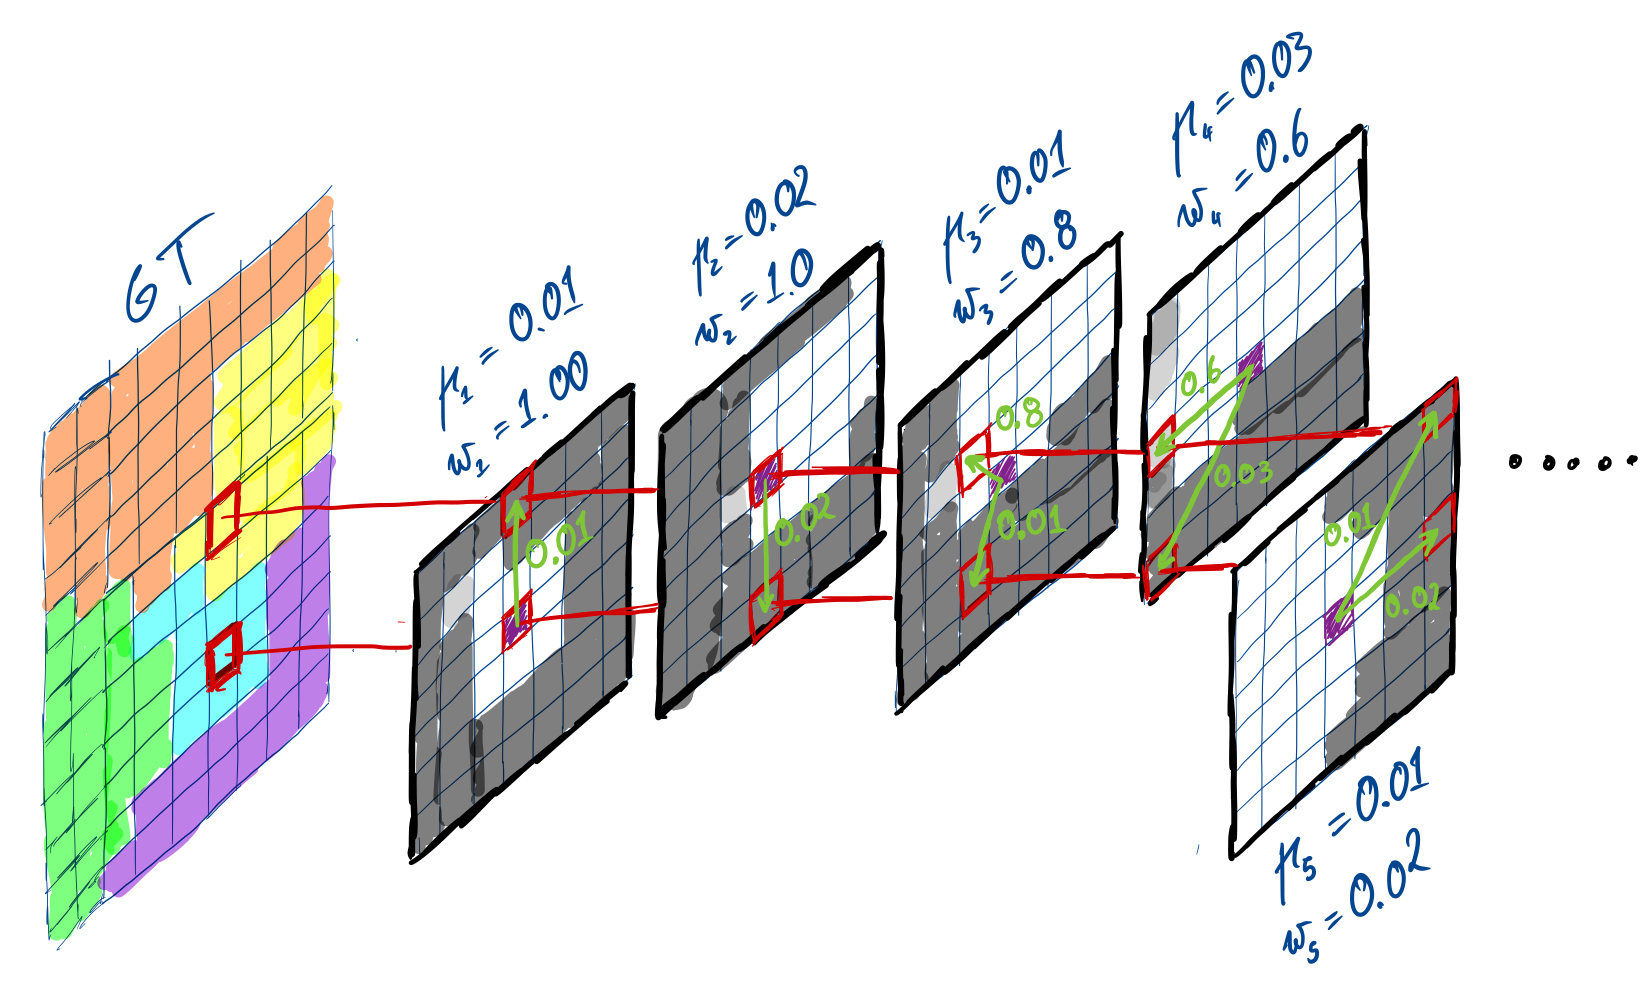
\includegraphics[width=0.7\textwidth]{./figs/alg_explaned.jpg} % 0.45
        \caption{Illustration of the proposed parameter-free method to convert self-probability masks to edge weights...}
    \label{fig:alg_explained}
\end{figure}
\begin{algorithm}[t]
  \begin{flushleft}
  \caption{: Computing affinities from self-probability masks}
   \hspace*{\algorithmicindent} \textbf{Input:} Graph $\mathcal{G}(V,E)$; local self-probability masks $\mathcal{M}_{\mathbf{x}}: \mathcal{N}_{K\times K} \rightarrow [0,1]$  \\
  \hspace*{\algorithmicindent} \textbf{Output:} Affinities $\bar{a}_e\in[0,1]$ with variance $\sigma^2_e$ for all edges $e\in E$\\
  \hspace*{\algorithmicindent} 
  \begin{algorithmic}[1]
  \footnotesize
  % \small
      % \State Initial clustering: $\Pi=\{\{v_1\}, \ldots, \{v_{|V|}\}\}$
      % \State Initialize interactions between clusters with $ = w^+_e - w^-_e$
      \For{each edge $e\in E$ in graph $\mathcal{G}$}
        \State Get coordinates $\mathbf{x}=(x_1,x_2)$ and $\mathbf{y}=(y_1,y_2)$ of pixels linked by edge $e$
        \State Init. accumulation sets $\mathcal{A}=\{\}$ for affinities and $\mathcal{W}=\{\}$ for reliability weights
        \For{each mask $\mathcal{M}_{\mathbf{c}}$ covering both pixel $\mathbf{x}$ and pixel $\mathbf{y}$}
            \State Get relative coords. $\delta_\mathbf{x}$ and $\delta_\mathbf{y}$ with respect to the center $\mathbf{c}$ of the mask $\mathcal{M}_{\mathbf{c}}$
            \State $\mathcal{A}\,\gets \mathcal{A} \,\cup\,\{\min \big(\mathcal{M}_{\mathbf{c}}(\delta_\mathbf{x}), \,\mathcal{M}_{\mathbf{c}}(\delta_\mathbf{y})\big)\}$ \Comment{Fuzzy-AND: both values active}
            \State $\mathcal{W}\gets \mathcal{W} \,\cup\,\{\max \big(\mathcal{M}_{\mathbf{c}}(\delta_\mathbf{x}), \,\mathcal{M}_{\mathbf{c}}(\delta_\mathbf{y})\big)\}$ \Comment{Fuzzy-OR: at least one value active}
        \EndFor
        \State Get weighted average $\bar{a}_e= (\sum_{a\in\mathcal{A}}\sum_{w\in\mathcal{W}} \,w\cdot a)\,/\,(\sum_{w\in\mathcal{W}}\,w)$ 
        \State Get weighted variance $\sigma^2_e = \big(\sum_{a\in\mathcal{A}}\sum_{w\in\mathcal{W}} \,w\cdot (a-\bar{a}_e)^2\big)\,/\,\big(\sum_{w\in\mathcal{W}}\,w\big)$
      \EndFor
      \State
      \Return $a_e, \sigma^2_e$ for each $e\in E$
  \end{algorithmic}
    \label{computing_affinities}
  \end{flushleft}

\end{algorithm}

\section{Computing affinities from self-probability masks}

\cite{liu2016multi} \emph{The patch pair with the highest overlap score is selected where corresponding segment masks are merged. This process iterates until no existing patch pair has the overlap score higher than a given threshold. Different scales are treated independently and duplicates are handled via non-max suppression}

\TODO{To be completed}
% A lot of recently proposed instance-segmentation methods, predict pairwise affinity between pairs of pixels 
By predicting a self-probability mask for each pixel, the pairwise affinity between two pixels is predicted 


One common used method is to predict a set of sparse affinities for every pixel (see Fig. \ref{fig:comparing_masks_affs}c)... 
These can then be see as edge weights of a grid-graph where each node represents a pixel of the image. And a graph clustering algorithm is then applied to output an instance segmentation.
In this section, we propose to ways to perform something similar and use the predicted per-pixel self-probability masks to define the edge weights of a grid-graph.
First, in Sec. \ref{sec:efficient_affs} we propose a simple way to efficiently extract a set of sparse affinities from the predicted encoded self-probability masks, without the need to decode them one by one. Then, in Sec. \ref{sec:prob_affs}...

\subsection{Efficient computation of sparse affinities from encoded masks}\label{sec:efficient_affs}
A commonly used instance segmentation method predicts, for each pixel, a small set of sparse short- and long-range affinities representing how likely it is for a pair of pixels to belong to the same object instance (see Fig. \ref{fig:comparing_masks_affs}c).



As a second contribution, we propose two distinct ways of converting the predicted per-pixel self-probability masks into edge weights of a graph representing the image, so that each node corresponds to a pixel and a graph clustering algorithm is then used to output an instance segmentation.

Here it would be nice to claim that hopefully the set of affinities we get out of this leads to more consistent neighborhood structures as compared to directly predicting each affinity as an output channel of the main model

\subsection{Averaged }\label{sec:prob_affs}
\begin{itemize}
\item Every patch predicts $M\times N$ affinities between the central pixel and the neighboring ones. But can we do better?
\item Defining the graph: we have an edge between two nodes $(i, j)$ only if $j \in M\times N$ Given two pixels  
\end{itemize}
- 


The second proposed method yields a parameter-free algorithm achieving competitive performances, yada yada yada... 





% !TEX root = ../patchEmbeddings_review.tex

\section{Experiments on neuron segmentation}
We first evaluate and compare our method on the task of neuron segmentation in electron microscopy (EM) image volumes. This application is of key interest in connectomics, a field of neuro-science with the goal of reconstructing neural wiring diagrams spanning complete central nervous systems. Currently, only proof-reading or manual tracing yields sufficient accuracy for correct circuit reconstruction \cite{schlegel2017learning}, thus further progress is required in automated reconstruction methods.

EM segmentation is commonly performed by first predicting 
boundary pixels \cite{beier2017multicut,ciresan2012deep} or undirected affinities \cite{wolf2018mutex,lee2017superhuman,funke2018large}, which represent how likely it is for a pair of pixels to belong to the same neuron segment. 

\TODO{Recap of what we do}

\subsection{Data: CREMI challenge} \label{sec:cremi_challenge}
We evaluate the proposed method on the competitive CREMI 2016 EM Segmentation Challenge \cite{cremiChallenge} that is currently the neuron segmentation challenge with the largest amount of training data available. The dataset comes from serial section EM of \emph{Drosophila} fruit-fly tissue and consists of 6 volumes of 1250x1250x125 voxels at resolution 4x4x40nm, three of which come with publicly available training ground truth. The results submitted to the leaderboard are evaluated using the CREMI score, which is given by the geometric mean of Variation of Information Score (VOI split + VOI merge \cite{arganda2015crowdsourcing}) and Adapted Rand-Score (Rand-Score), two popular metrics used to evaluate clusterings.\\

The data from the CREMI challenge is highly anisotropic and contains artifacts like missing sections, staining precipitations and support film folds. 
To alleviate difficulties stemming from misalignment, we use a version of the data that was elastically realigned by the challenge organizers with the method of \cite{saalfeld2012elastic}.
We train a 3D U-Net \cite{ronneberger2015u, cciccek20163d} \UPDATE{using the same architecture as \cite{funke2018large} and predict long-and-short range affinities 
as described in \cite{lee2017superhuman}}. In addition to the standard data augmentation techniques of random rotations, random flips and  elastic deformations, we simulate data artifacts.
In more detail, we randomly zero-out slices, decrease the contrast of slices, simulate tears, introduce alignment jitter and paste artifacts extracted from the training data. Both \cite{funke2018large} and \cite{lee2017superhuman} have shown
that these kinds of augmentations can help to alleviate issues caused by EM-imaging artifacts.
We use Adam optimizer to train the network. The model was trained on all the three samples with available ground truth labels.  

\subsubsection{Predicting glia neurons}


% !TEX root = ../patchEmbeddings_review.tex

\section{Conclusions}
\begin{itemize}
\item Use predicted uncertainty in clustering algorithm
\end{itemize}




\clearpage
% ---- Bibliography ----
%
% BibTeX users should specify bibliography style 'splncs04'.
% References will then be sorted and formatted in the correct style.
%
\bibliographystyle{splncs04}
\bibliography{patchEmbeddings}

\newpage
% !TEX root = ../patchEmbeddings_review.tex

\renewcommand{\thesection}{S\arabic{section}}
\renewcommand{\thetable}{S\arabic{table}}
\renewcommand{\thefigure}{S\arabic{figure}}

\section{Supplementary material}
% \subsection{Averaging overlapping masks}
% In Sec. \ref{sec:aggr_affs}, we introduce a parameter-free algorithm \ref{alg:computing_affinities} to average overlapping masks and extract affinities that can be then used as edge weights of a signed graph with both positive and negative weights. 

% In Fig. \ref{fig:alg_explained}, we show a simplified example of how Algorithm \ref{alg:computing_affinities} computes affinities between a pair of pixels $u$ and $v$.
% In Fig. \ref{fig:mask_cases}, we list the cases in which a \maskname mask can be used or not to predict the affinity between two pixels belonging to the mask.  
% In Fig. \ref{fig:affs_comparison} we compare affinities predicted either by averaging \maskname masks or by directly predicting them as a binary classification output of the model trained with a dense channel-wise S\o rensen-Dice loss.

% Algorithm \ref{alg:computing_affinities} is efficiently implemented on GPU by making use of the \texttt{fold} and \texttt{unfold} functions in PyTorch \cite{NEURIPS2019_9015}. 


\subsection{Graph neighborhood structure and output instance segmentation}
In the first column of Table \ref{tab:neighborhood_structures}, we provide the neighborhood structure of the pixel grid-graph, which is very similar to the one used in related work \cite{wolf2018mutex,lee2017superhuman}.
In Fig. \ref{fig:MWS_segm}, we show the resulting instance segmentation obtained by computing affinities from \maskname masks and then running the Mutex Watershed algorithm on the obtained graph with positive and negative edge weights.

\paragraph{Removing small segments} -- After running the Mutex Watershed, we use a simple post-processing step to delete small segments on the boundaries, most of which are given by single-voxel clusters. On the neuron segmentation predictions, we deleted all regions with less than 200 voxels and used a seeded watershed algorithm to expand the bigger segments.


\subsection{Details on the model architecture}\label{sec:arch_details_suppl}
Fig. \ref{fig:model_architecture} shows the details on the 3D-UNet architecture and Table \ref{tab:neighborhood_structures} lists the sparse neighborhood structures predicted by the \emph{\sparseBr branches}. Only the outputs at the highest resolution (given by branches SNB$_1$, ENB$_1$ and ENB$_2$) are used to compute edge weights in the pixel grid-graph. A visualization of the predicted single-instance mask latent spaces is given in Fig. \ref{fig:PCA_embeddings}.
% - Cite architecture figure Fig: we use three type of nets, we only use highest res predictions for computing affinities of the graph

The input volume has shape $272 \times 272\times12$ which is equivalent to a volume of $544\times 544\times 12$ voxels in the original resolution $4\times 4\times 40$ nm$^3$. Before to apply the loss, we crop the predictions to a shape $224\times 224\times 9$ in order to avoid border artifacts\footnote{Instead of cropping directly the final predictions, we perform several crops in the decoder part of the UNet model (see Upsample + Crop connections in Fig. \ref{fig:model_architecture}) in order to optimize GPU-memory usage.}.
The final model trained on all available ground truth labels is trained with a slightly larger input volume of $288\times 288\times 14$.



% \begin{itemize}
% \item residual blocks with group normalization layers and skip-connections involving sum of feature maps from 
% \item The input volume has shape $272 \times 272\times12$ which is equivalent to a volume of $544\times 544\times 12$ voxels in the original resolution $4\times 4\times 40$ nm$^3$. Before to apply the loss, we crop the predictions to a shape $224\times 224\times 9$ in order to avoid border artifacts. 
% The final model trained on all available ground truth labels is trained with a slightly larger input volume of $288\times 288\times 14$ and we provide even more input to the cheaper glia-predictor-model: $352\times 352\times 15$ voxels. 
% \item Explicitly say what is the size of the coarsest predicted mask in the original res, which should be $112 \times 112 \times 5$ voxels at res...
% \item which outputs do we use for the averaging stuff? Only the high-res ones
% \item Crops in the decoder part
% \item In the supplementary material, we provide all the architecture details: crops in the decoder of the UNet
% \item we predict two types of \maskname masks at the highest level of the hierarchy
% \item Post-processing (remove small segments)
% \item we only use the outputs at the highest resolution for predicting affinities!
% \item we either use all, only SNB or only ENB
% \end{itemize}






% \textbf{Glia classifier} -- As a final post-processing step, we merge neighboring instances that have been classified as \emph{glia segments} (putative astrocyte). This is a common procedure in neuron segmentation \TODO{CIT}\cite{lee2019learning}, since glia segments are substantially different from the other neurons and are usually considered separately in the final reconstructed diagram of neural circuit connectivity. Glia segments usually present a main body with a lot of very thin glial processes




% \begin{figure}[t]
% \begin{subfigure}[t]{0.47\linewidth}
% \centering
% 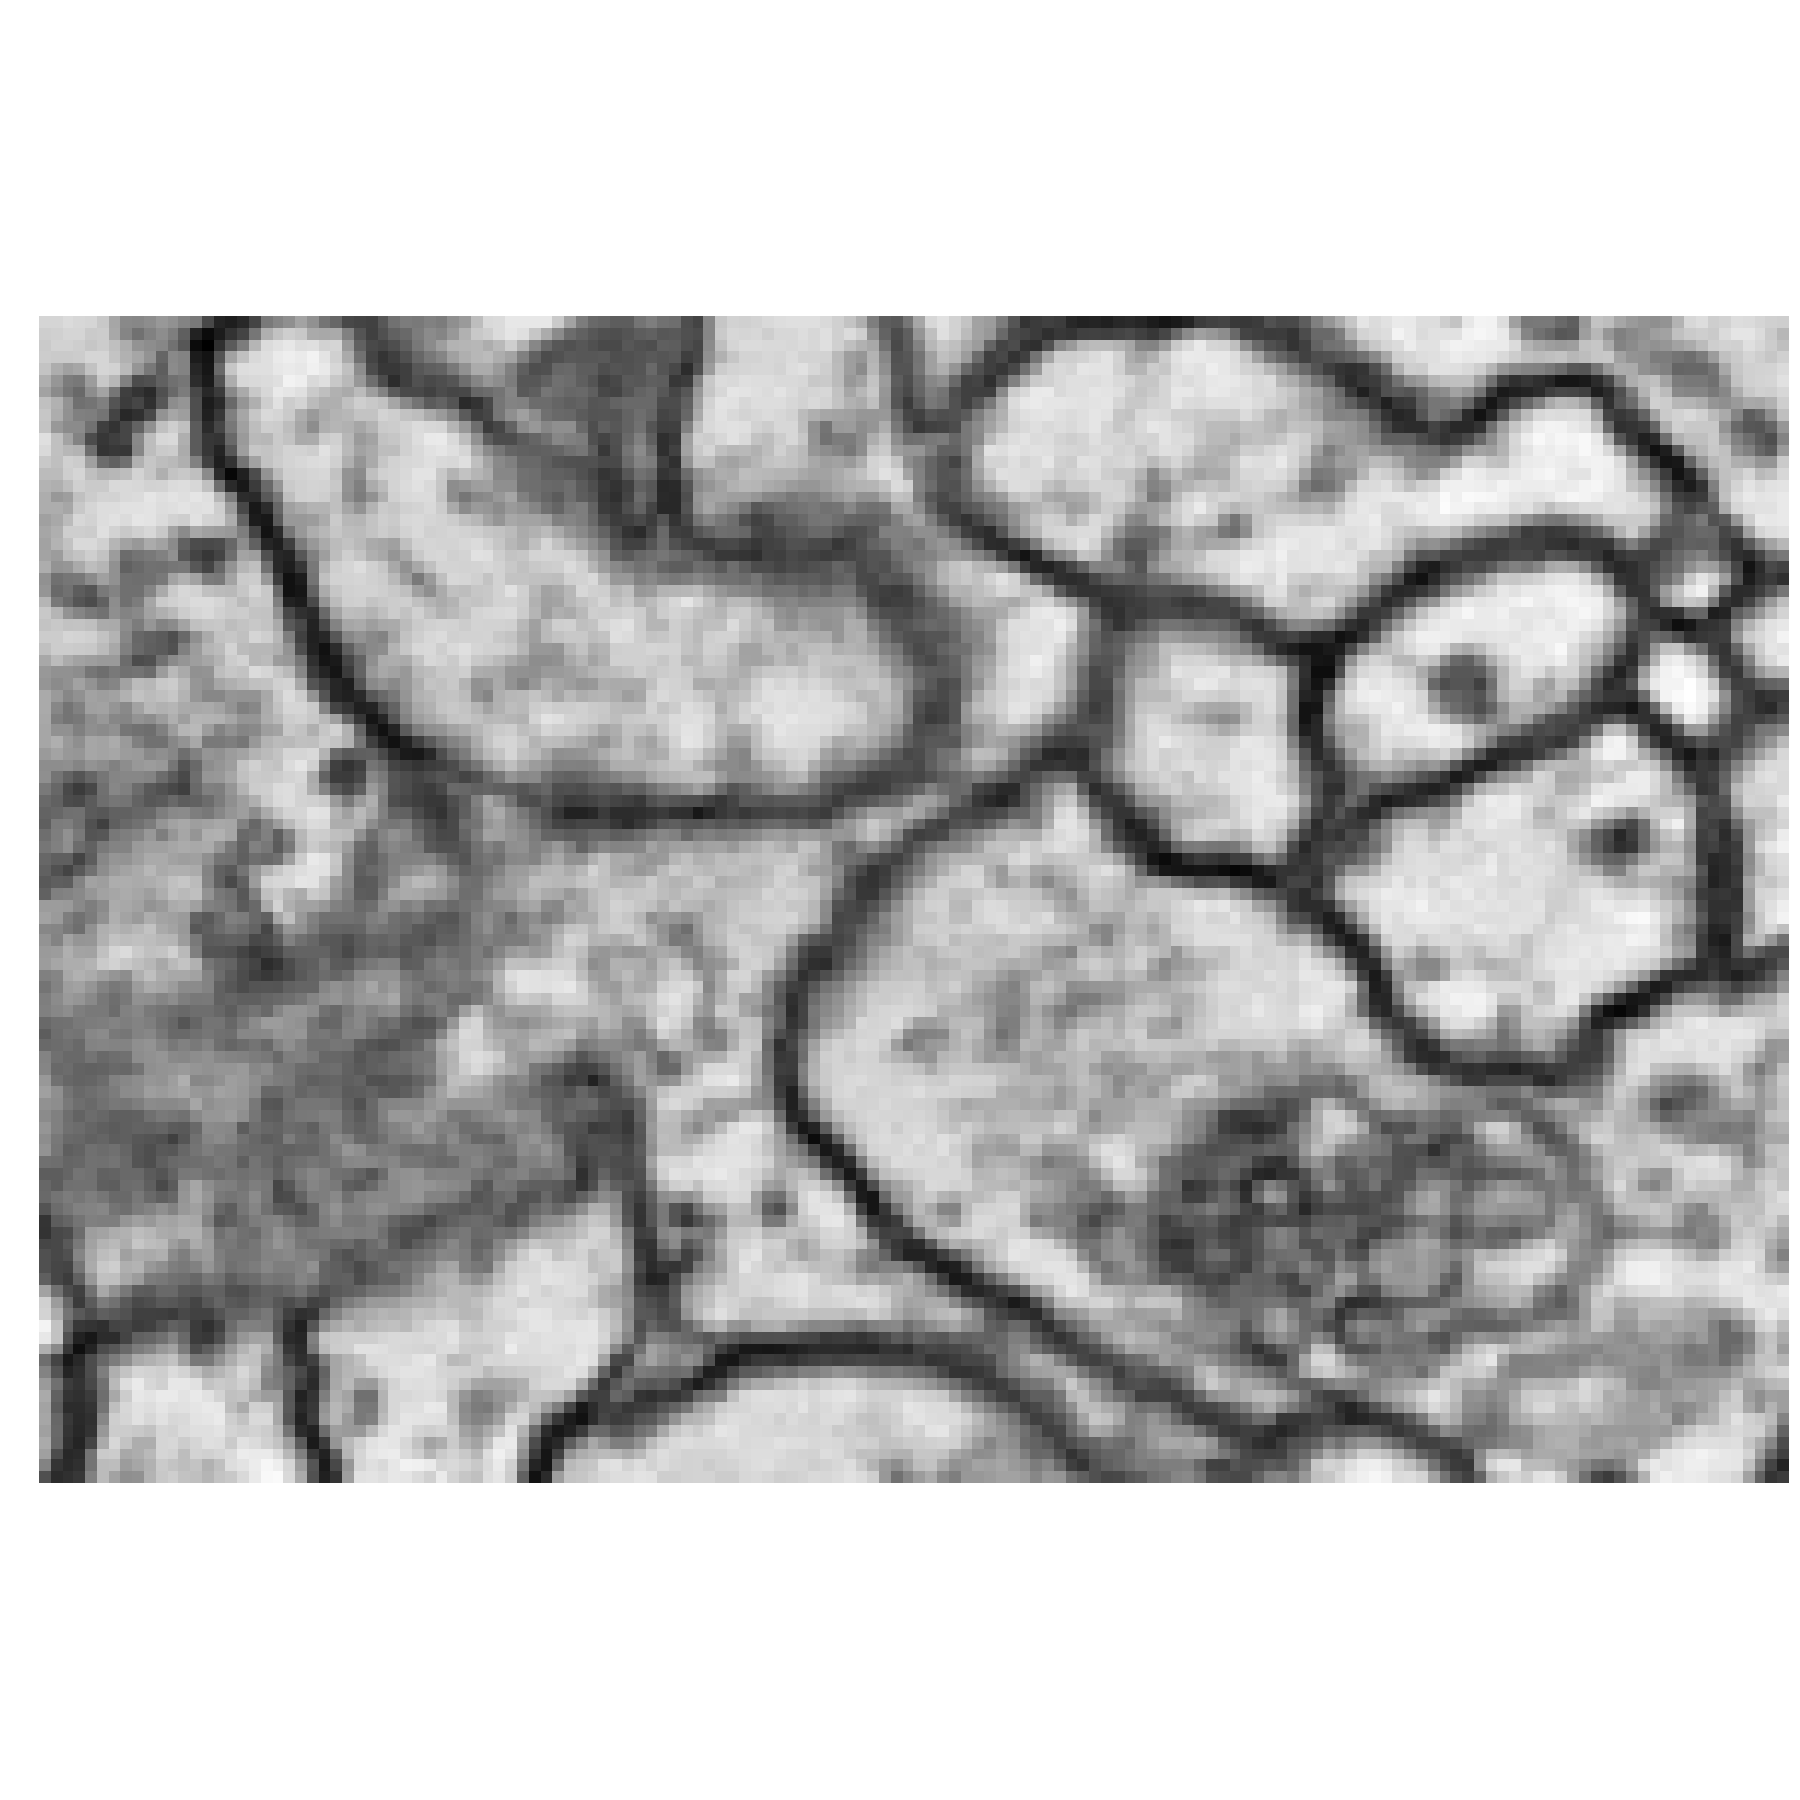
\includegraphics[width=0.65\linewidth,trim=1.50in 1.4in 1.4in 1.50in,clip]{./figs/affs_compare/raw_mod.pdf} % 
% \caption{\centering Raw image}
% \end{subfigure}\hfill
% \begin{subfigure}[t]{0.47\textwidth}
% \centering
% 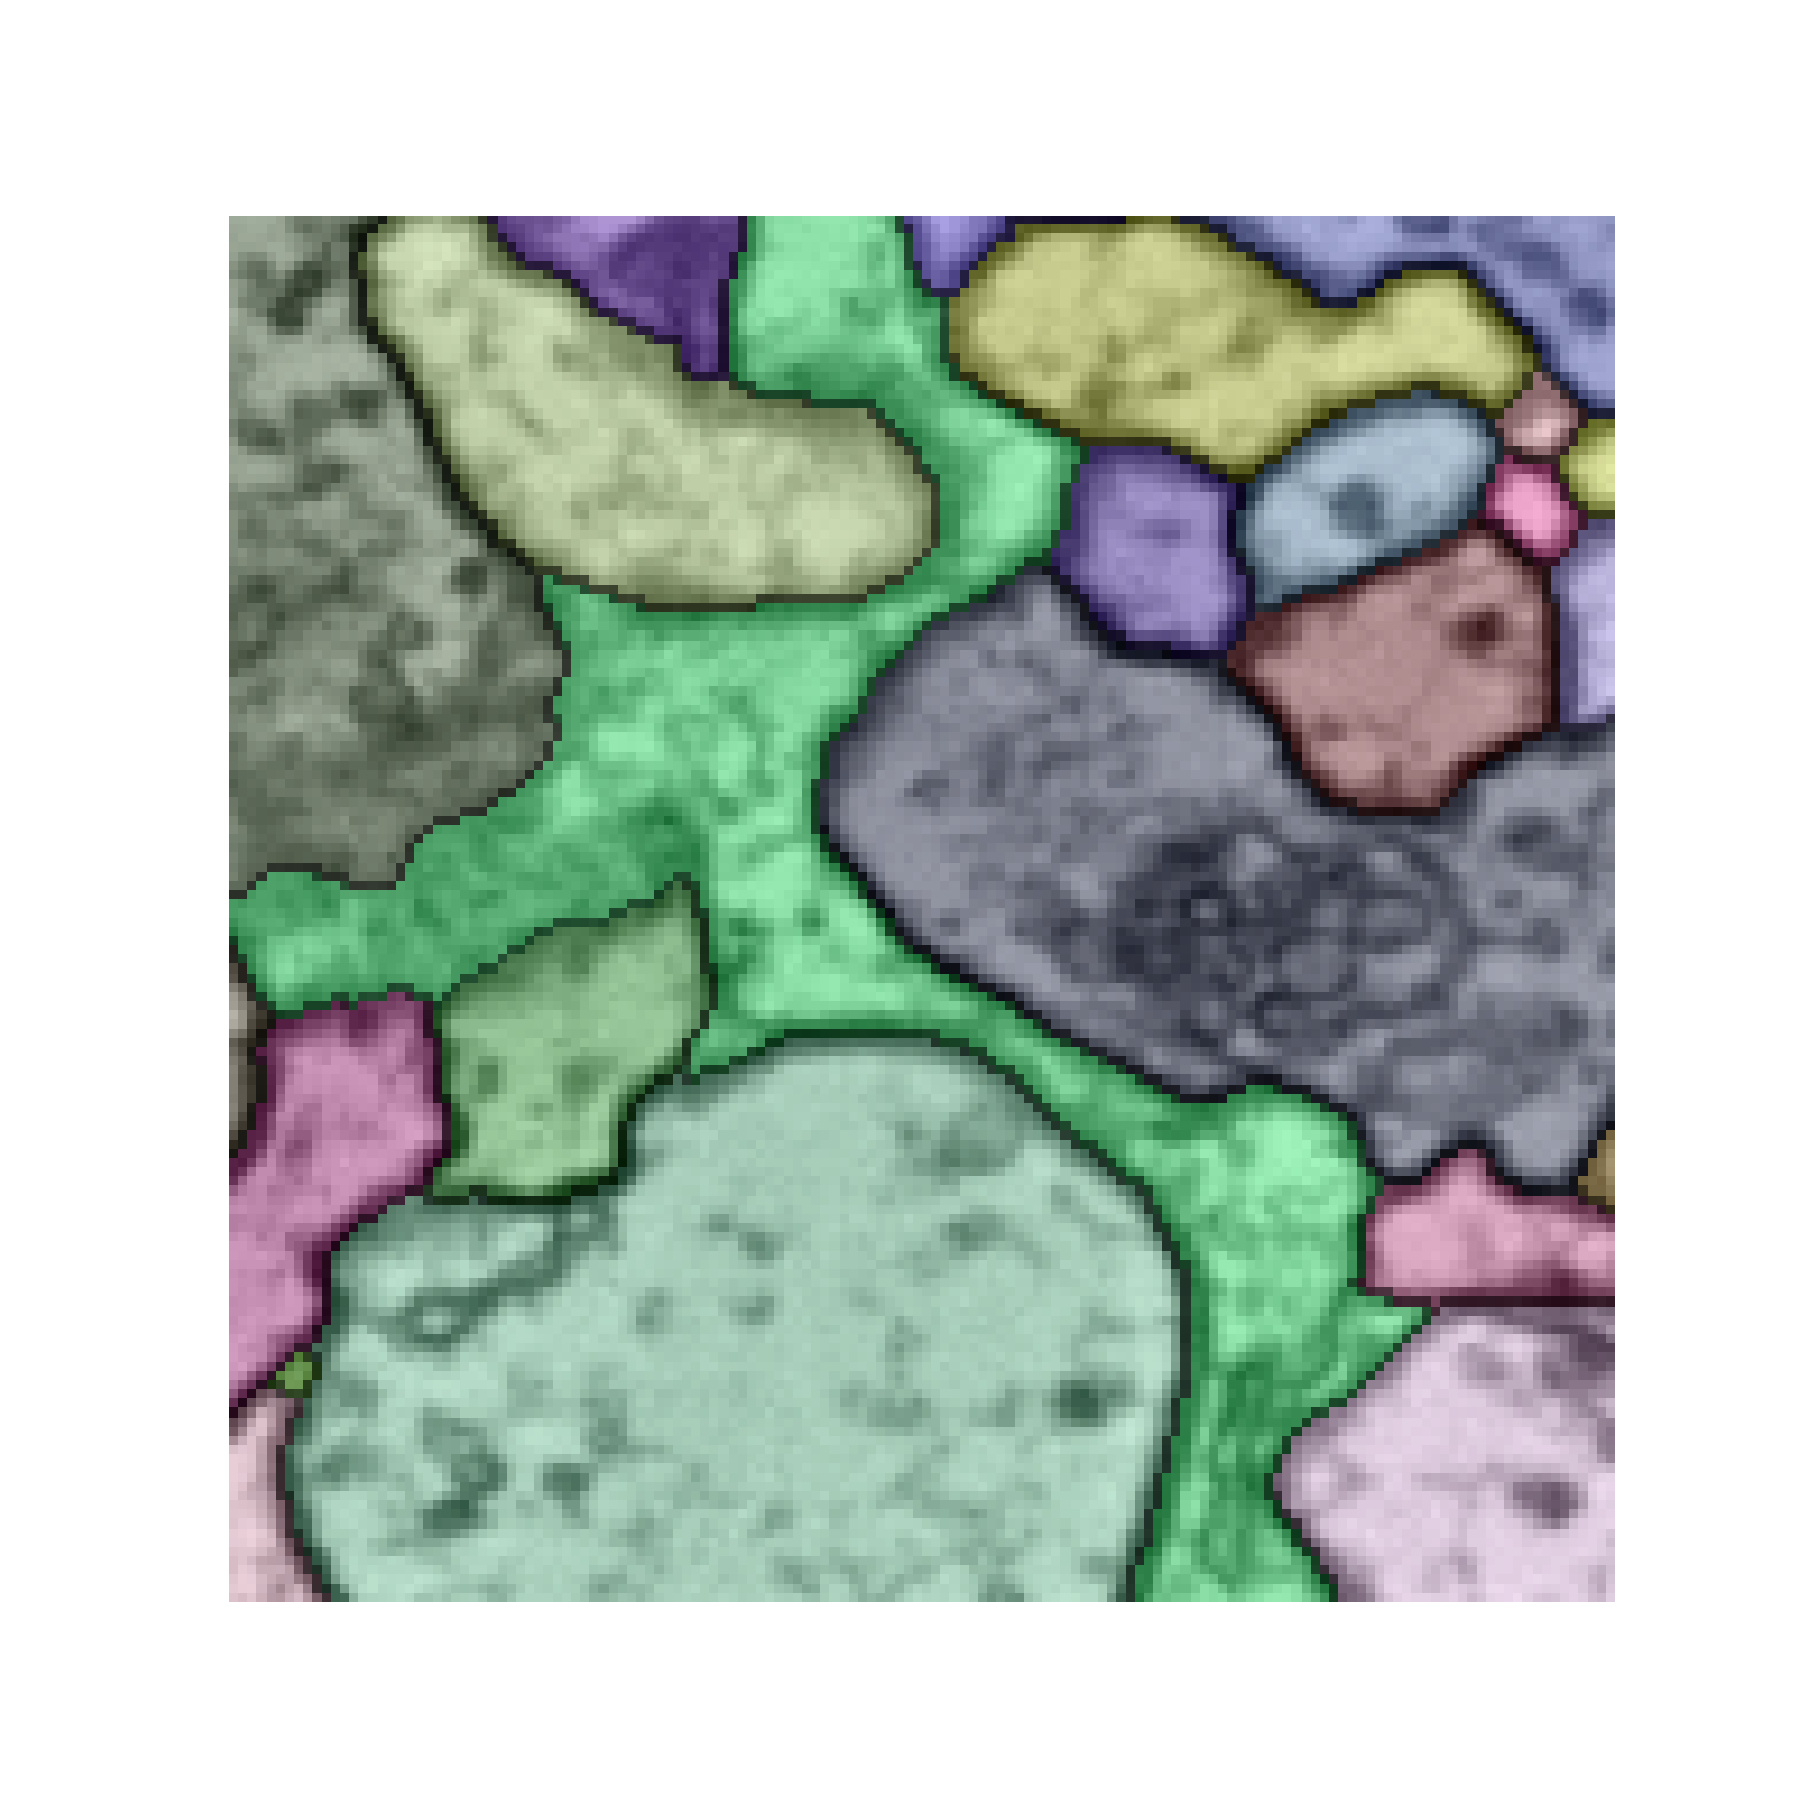
\includegraphics[width=0.65\linewidth,trim=1.50in 1.4in 1.4in 1.50in,clip]{./figs/affs_compare/GT.pdf} % ,trim=0.25in 0.25in 0.65in 0.36in,clip
% \caption{\centering Ground truth segmentation overlaid with the raw image}
% \end{subfigure}\vspace{2em}\\
% \begin{subfigure}[t]{0.47\linewidth}
% \centering
% 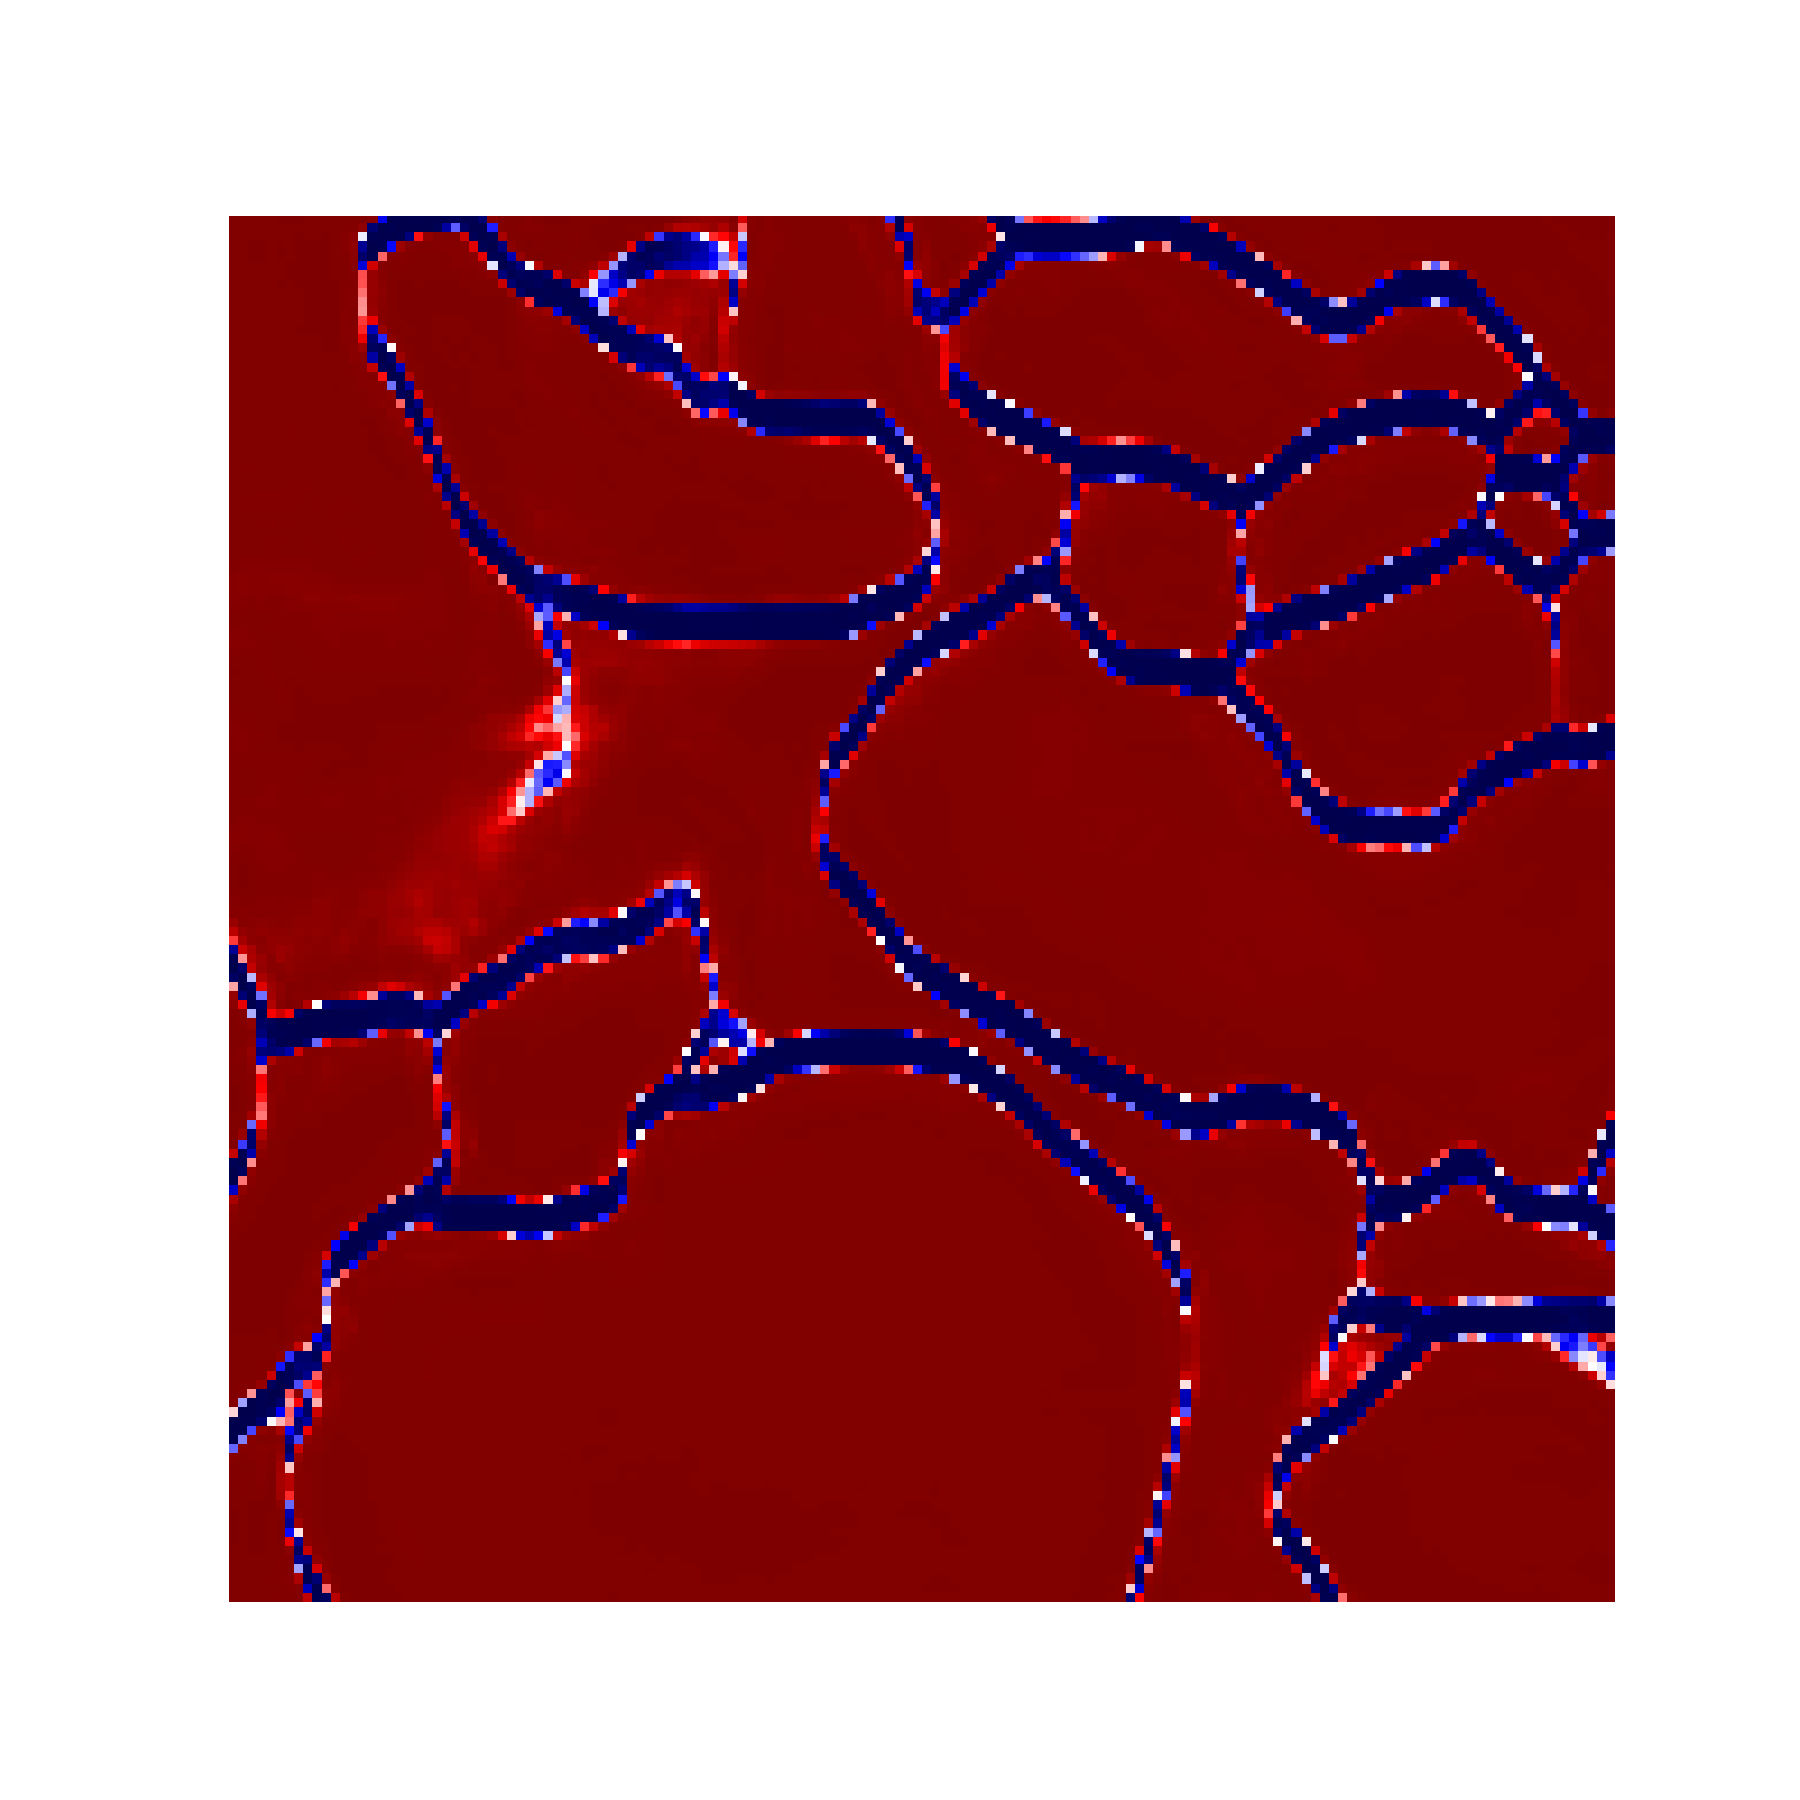
\includegraphics[width=0.65\linewidth,trim=1.50in 1.4in 1.4in 1.50in,clip]{./figs/affs_compare/affs1.pdf} % ,trim=0.25in 0.25in 0.65in 0.36in,clip
% \caption{\centering Affinities trained with S\o rensen-Dice loss (along vertical direction)}
% \end{subfigure}\hfill
% \begin{subfigure}[t]{0.47\textwidth}
% \centering
% 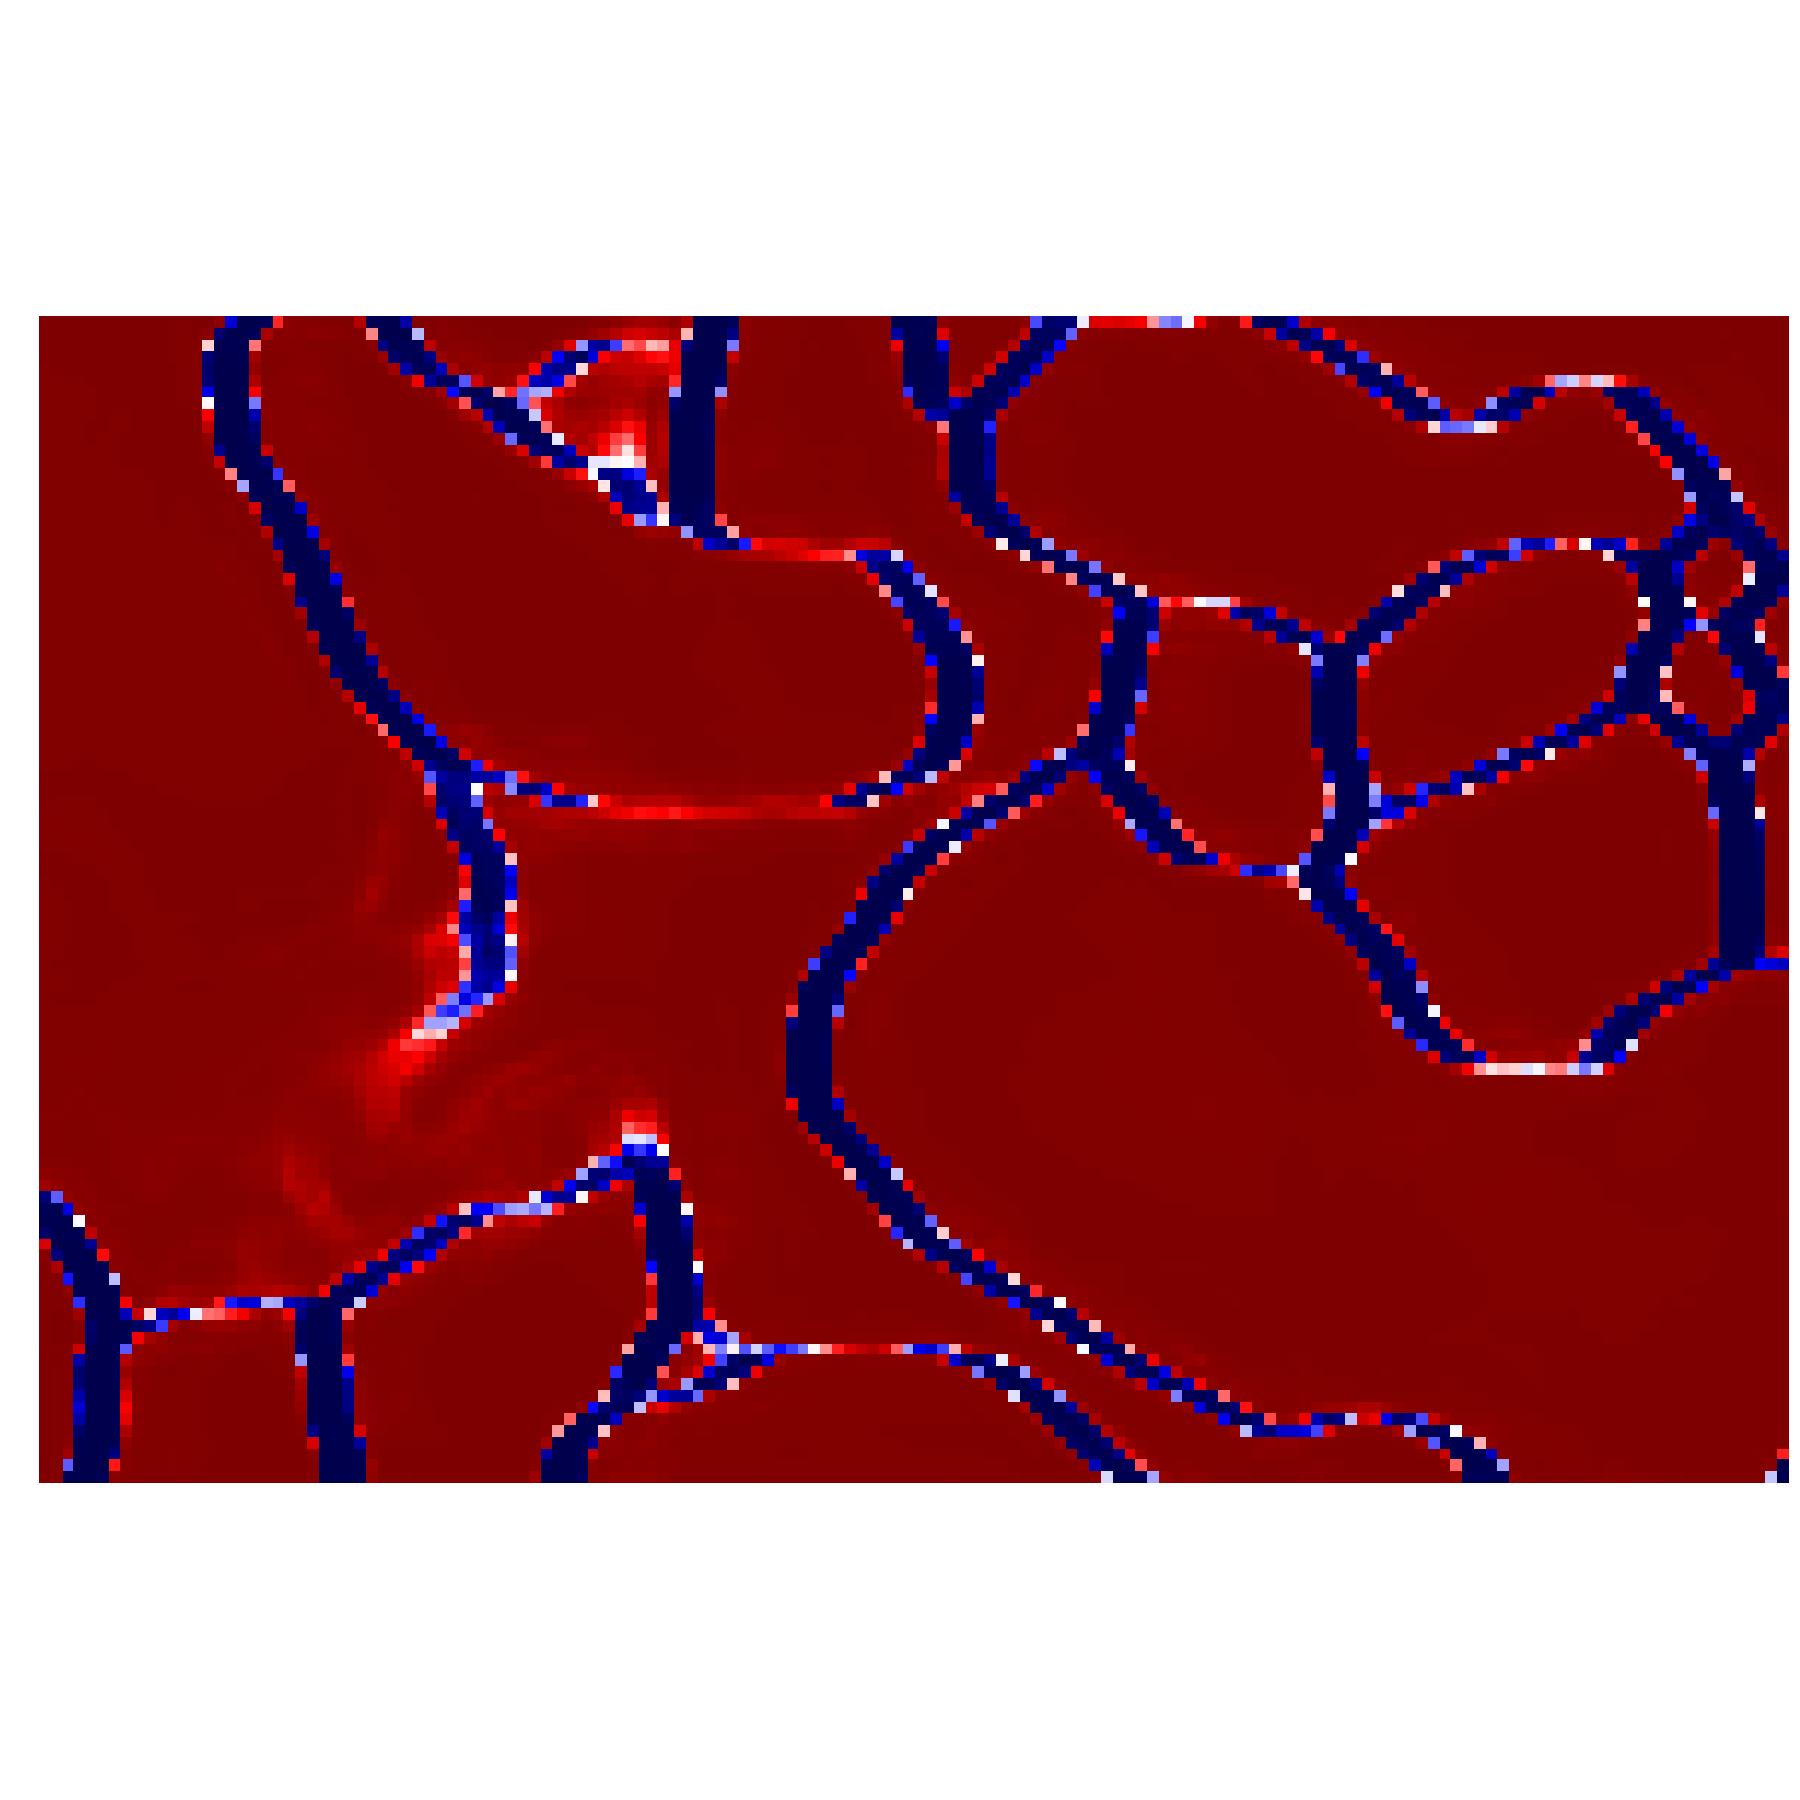
\includegraphics[width=0.65\linewidth,trim=1.50in 1.4in 1.4in 1.50in,clip]{./figs/affs_compare/affs2.pdf} % ,trim=0.25in 0.25in 0.65in 0.36in,clip
% \caption{\centering Affinities trained with S\o rensen-Dice loss (along horizontal direction)}
% \end{subfigure}\vspace{2em}\\
% \begin{subfigure}[t]{0.47\linewidth}
% \centering
% 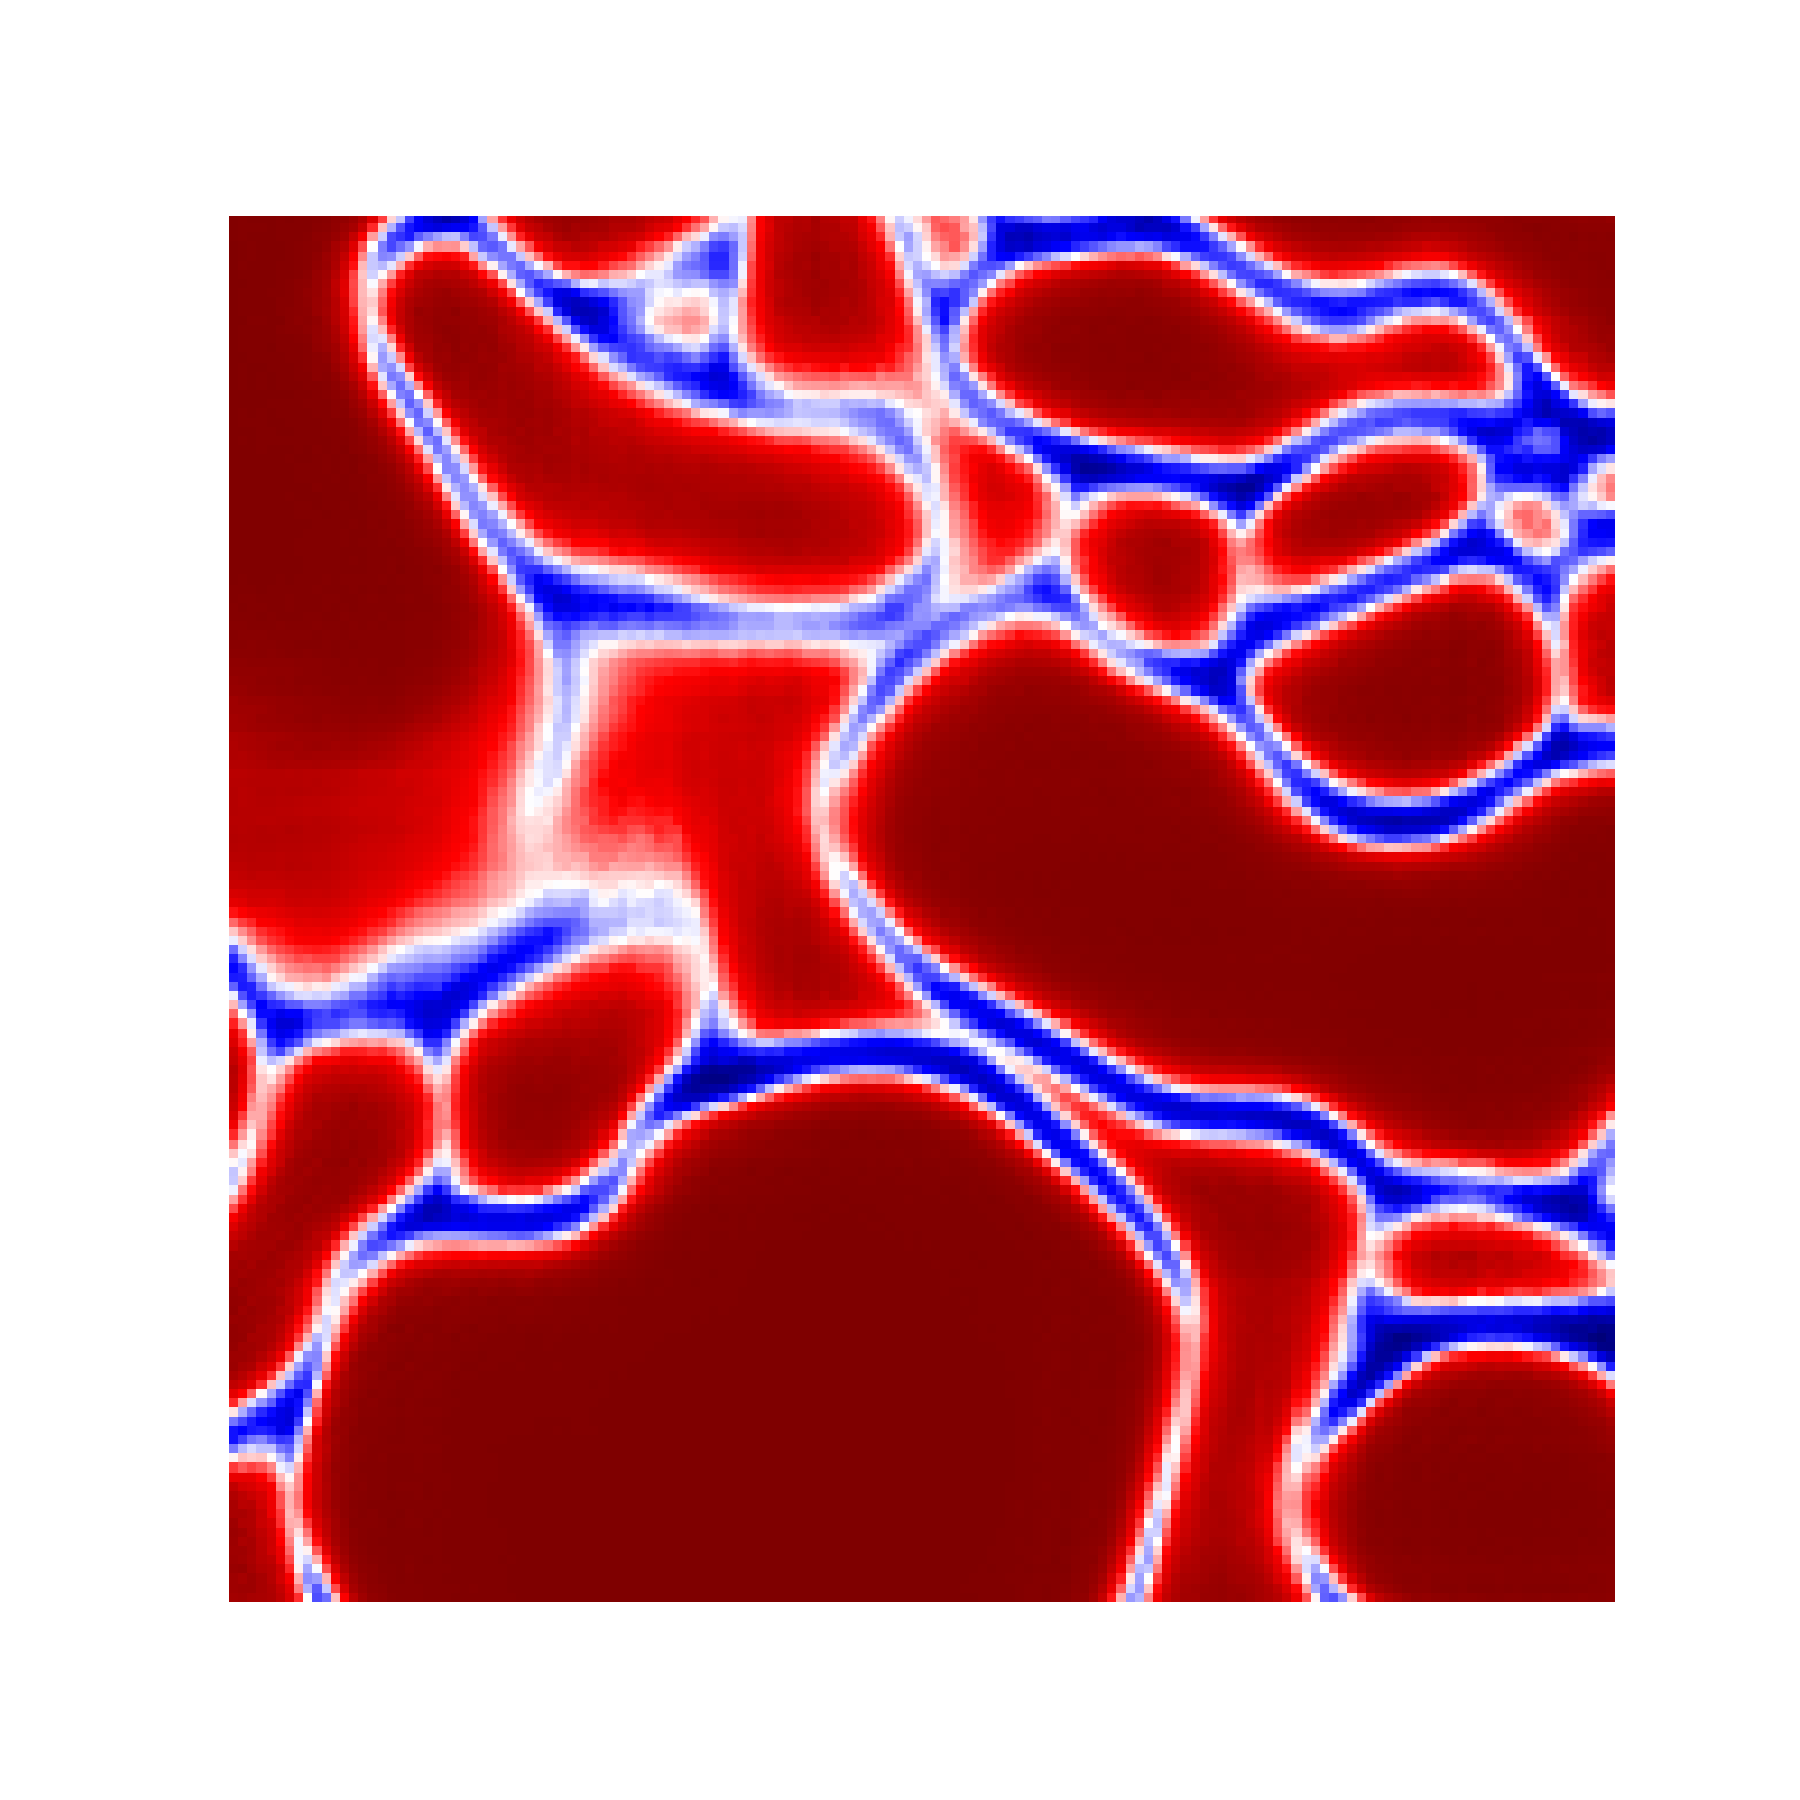
\includegraphics[width=0.65\linewidth,trim=1.50in 1.4in 1.4in 1.50in,clip]{./figs/affs_compare/affs3.pdf} % ,trim=0.25in 0.25in 0.65in 0.36in,clip
% \caption{\centering Affinities from averaging overlapping masks (along vertical direction)}
% \end{subfigure}\hfill
% \begin{subfigure}[t]{0.47\textwidth}
% \centering
% 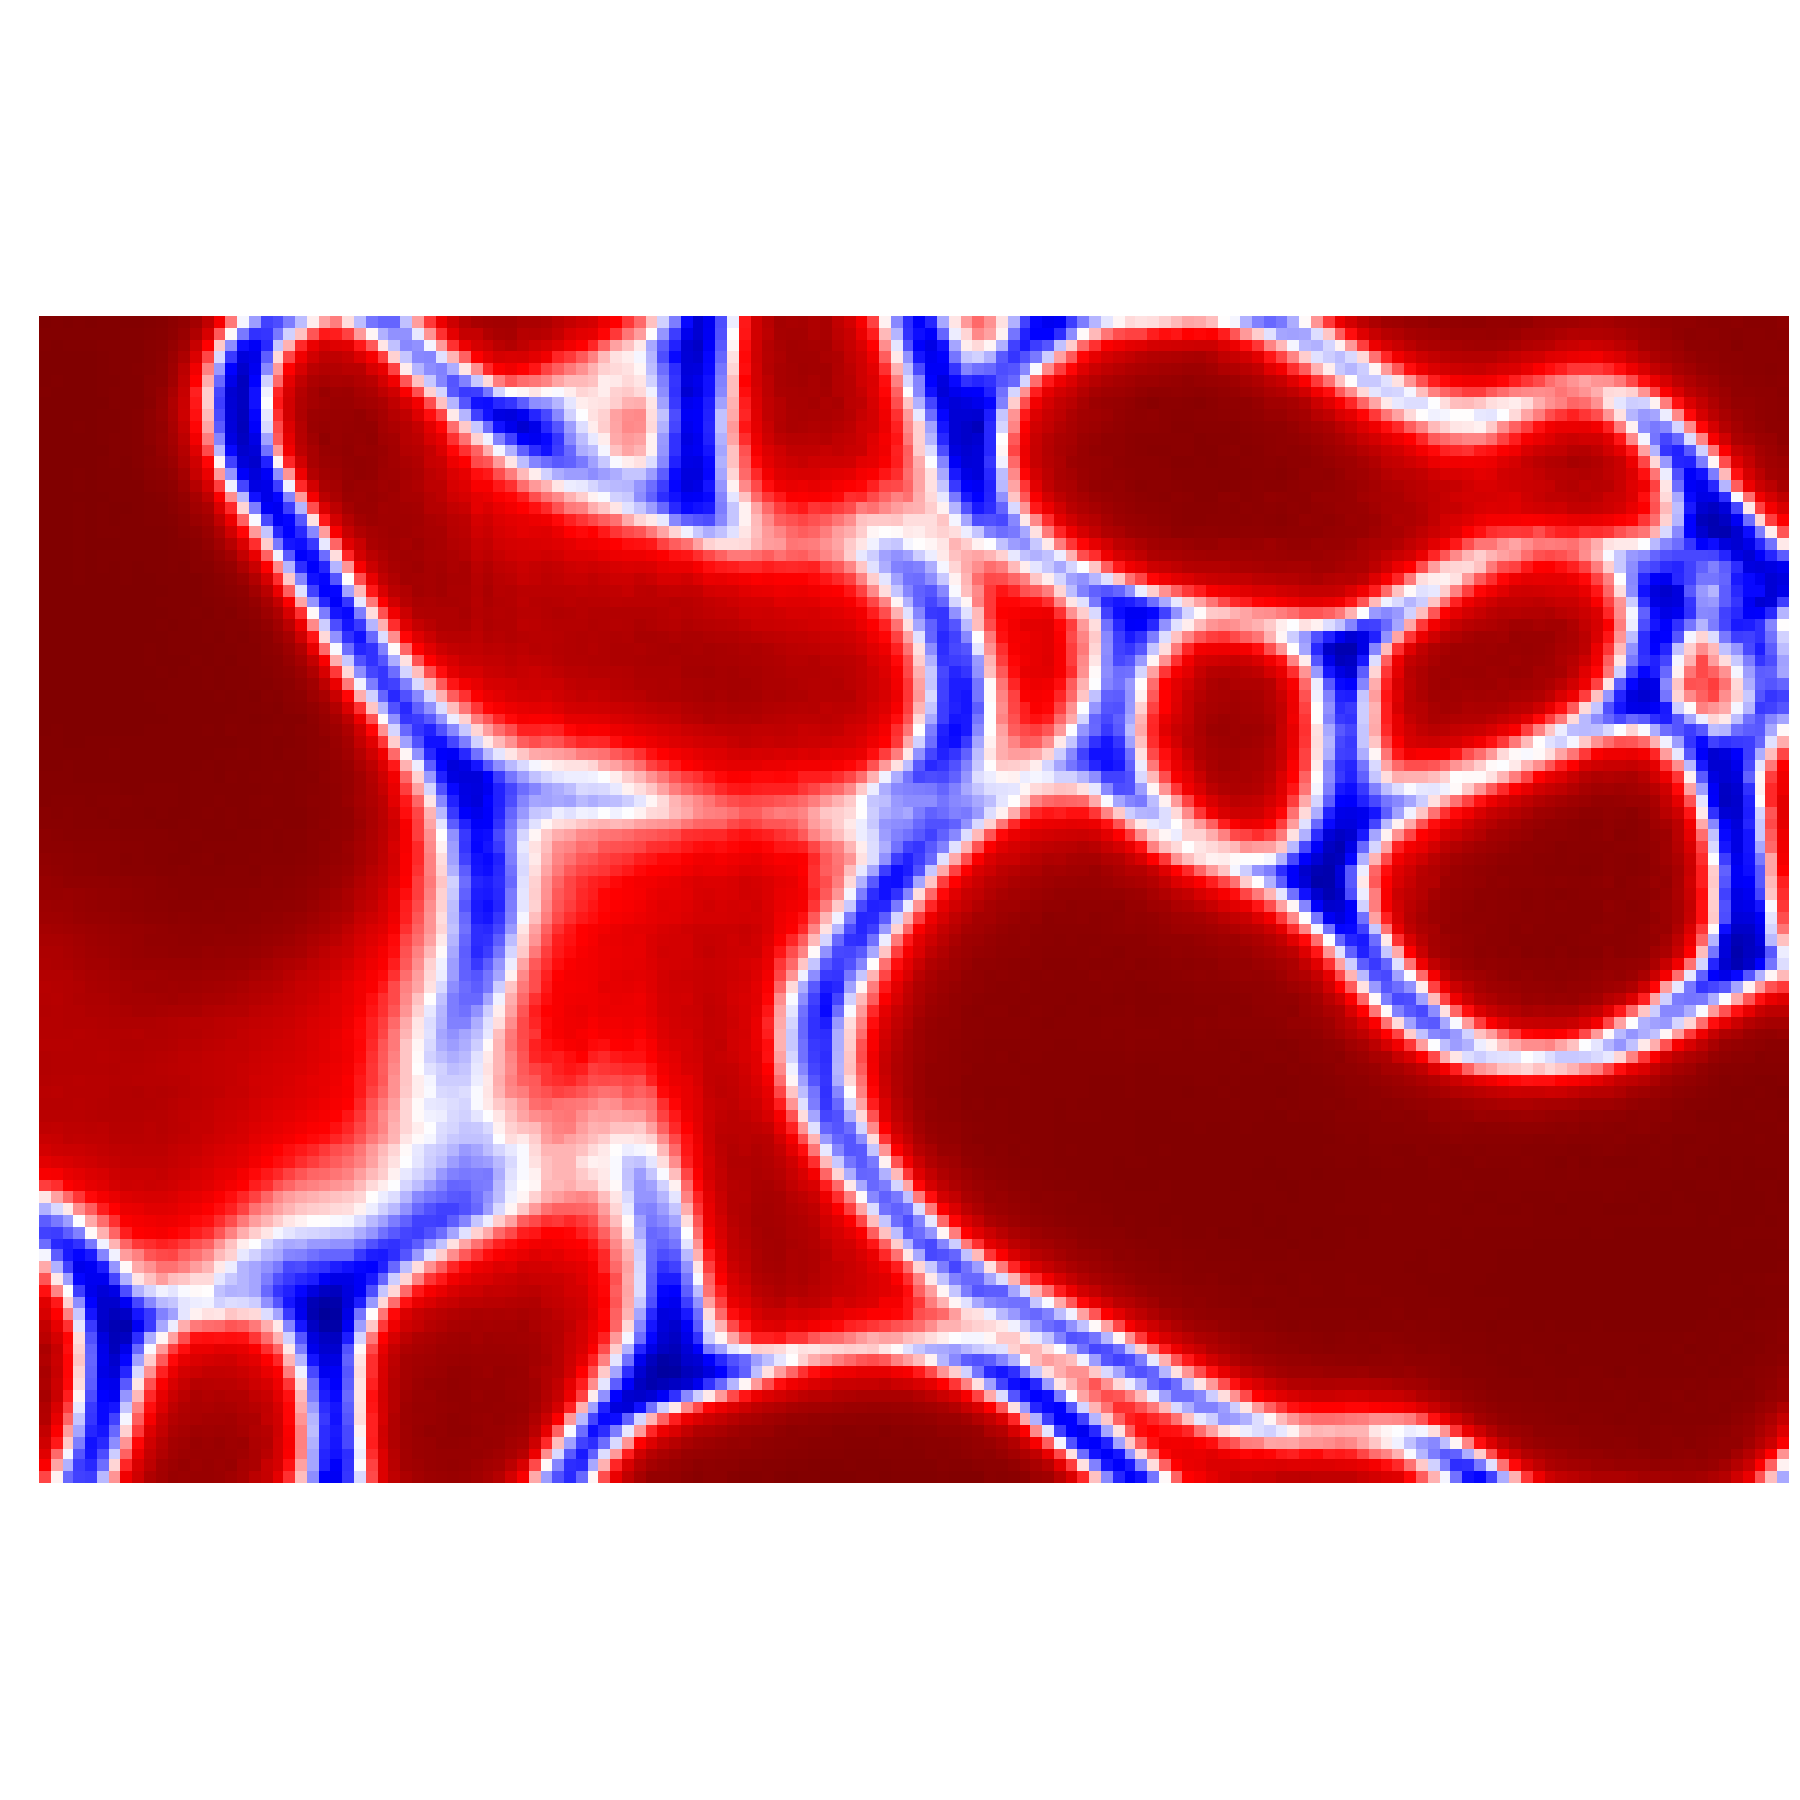
\includegraphics[width=0.65\linewidth,trim=1.50in 1.4in 1.4in 1.50in,clip]{./figs/affs_compare/affs4.pdf} % ,trim=0.25in 0.25in 0.65in 0.36in,clip
% \caption{\centering Affinities from averaging overlapping masks (along horizontal direction)}
% \end{subfigure}
% \caption{Comparison between different ways of predicting affinities and their robustness to noise. \textbf{(a-b)} Raw data and  associated ground-truth labels. \textbf{(c-d)} Affinities predicted by the \emph{sparse-neighborhood branch}, which is trained with a dense channel-wise S\o rensen-Dice loss (high affinities are represented in red, low ones in blue). \textbf{(e-f)} Affinities computed by averaging overlapping masks (AffAggr). We note how averaged affinities are smoother and present a more consistent boundary evidence in the noisy region highlighted by the red circle. In these plots we show two types of affinities representing neighborhood relations along the horizontal (-4, 0, 0) and vertical (0, -4, 0) directions.}\label{fig:affs_comparison}
% \end{figure}

\begin{figure}[t]
\centering
        % \includegraphics[width=0.4\textwidth,trim=0.25in 0.25in 0.68in 0.36in,clip]{./figs/SSBM_experiments.pdf} % 0.45
        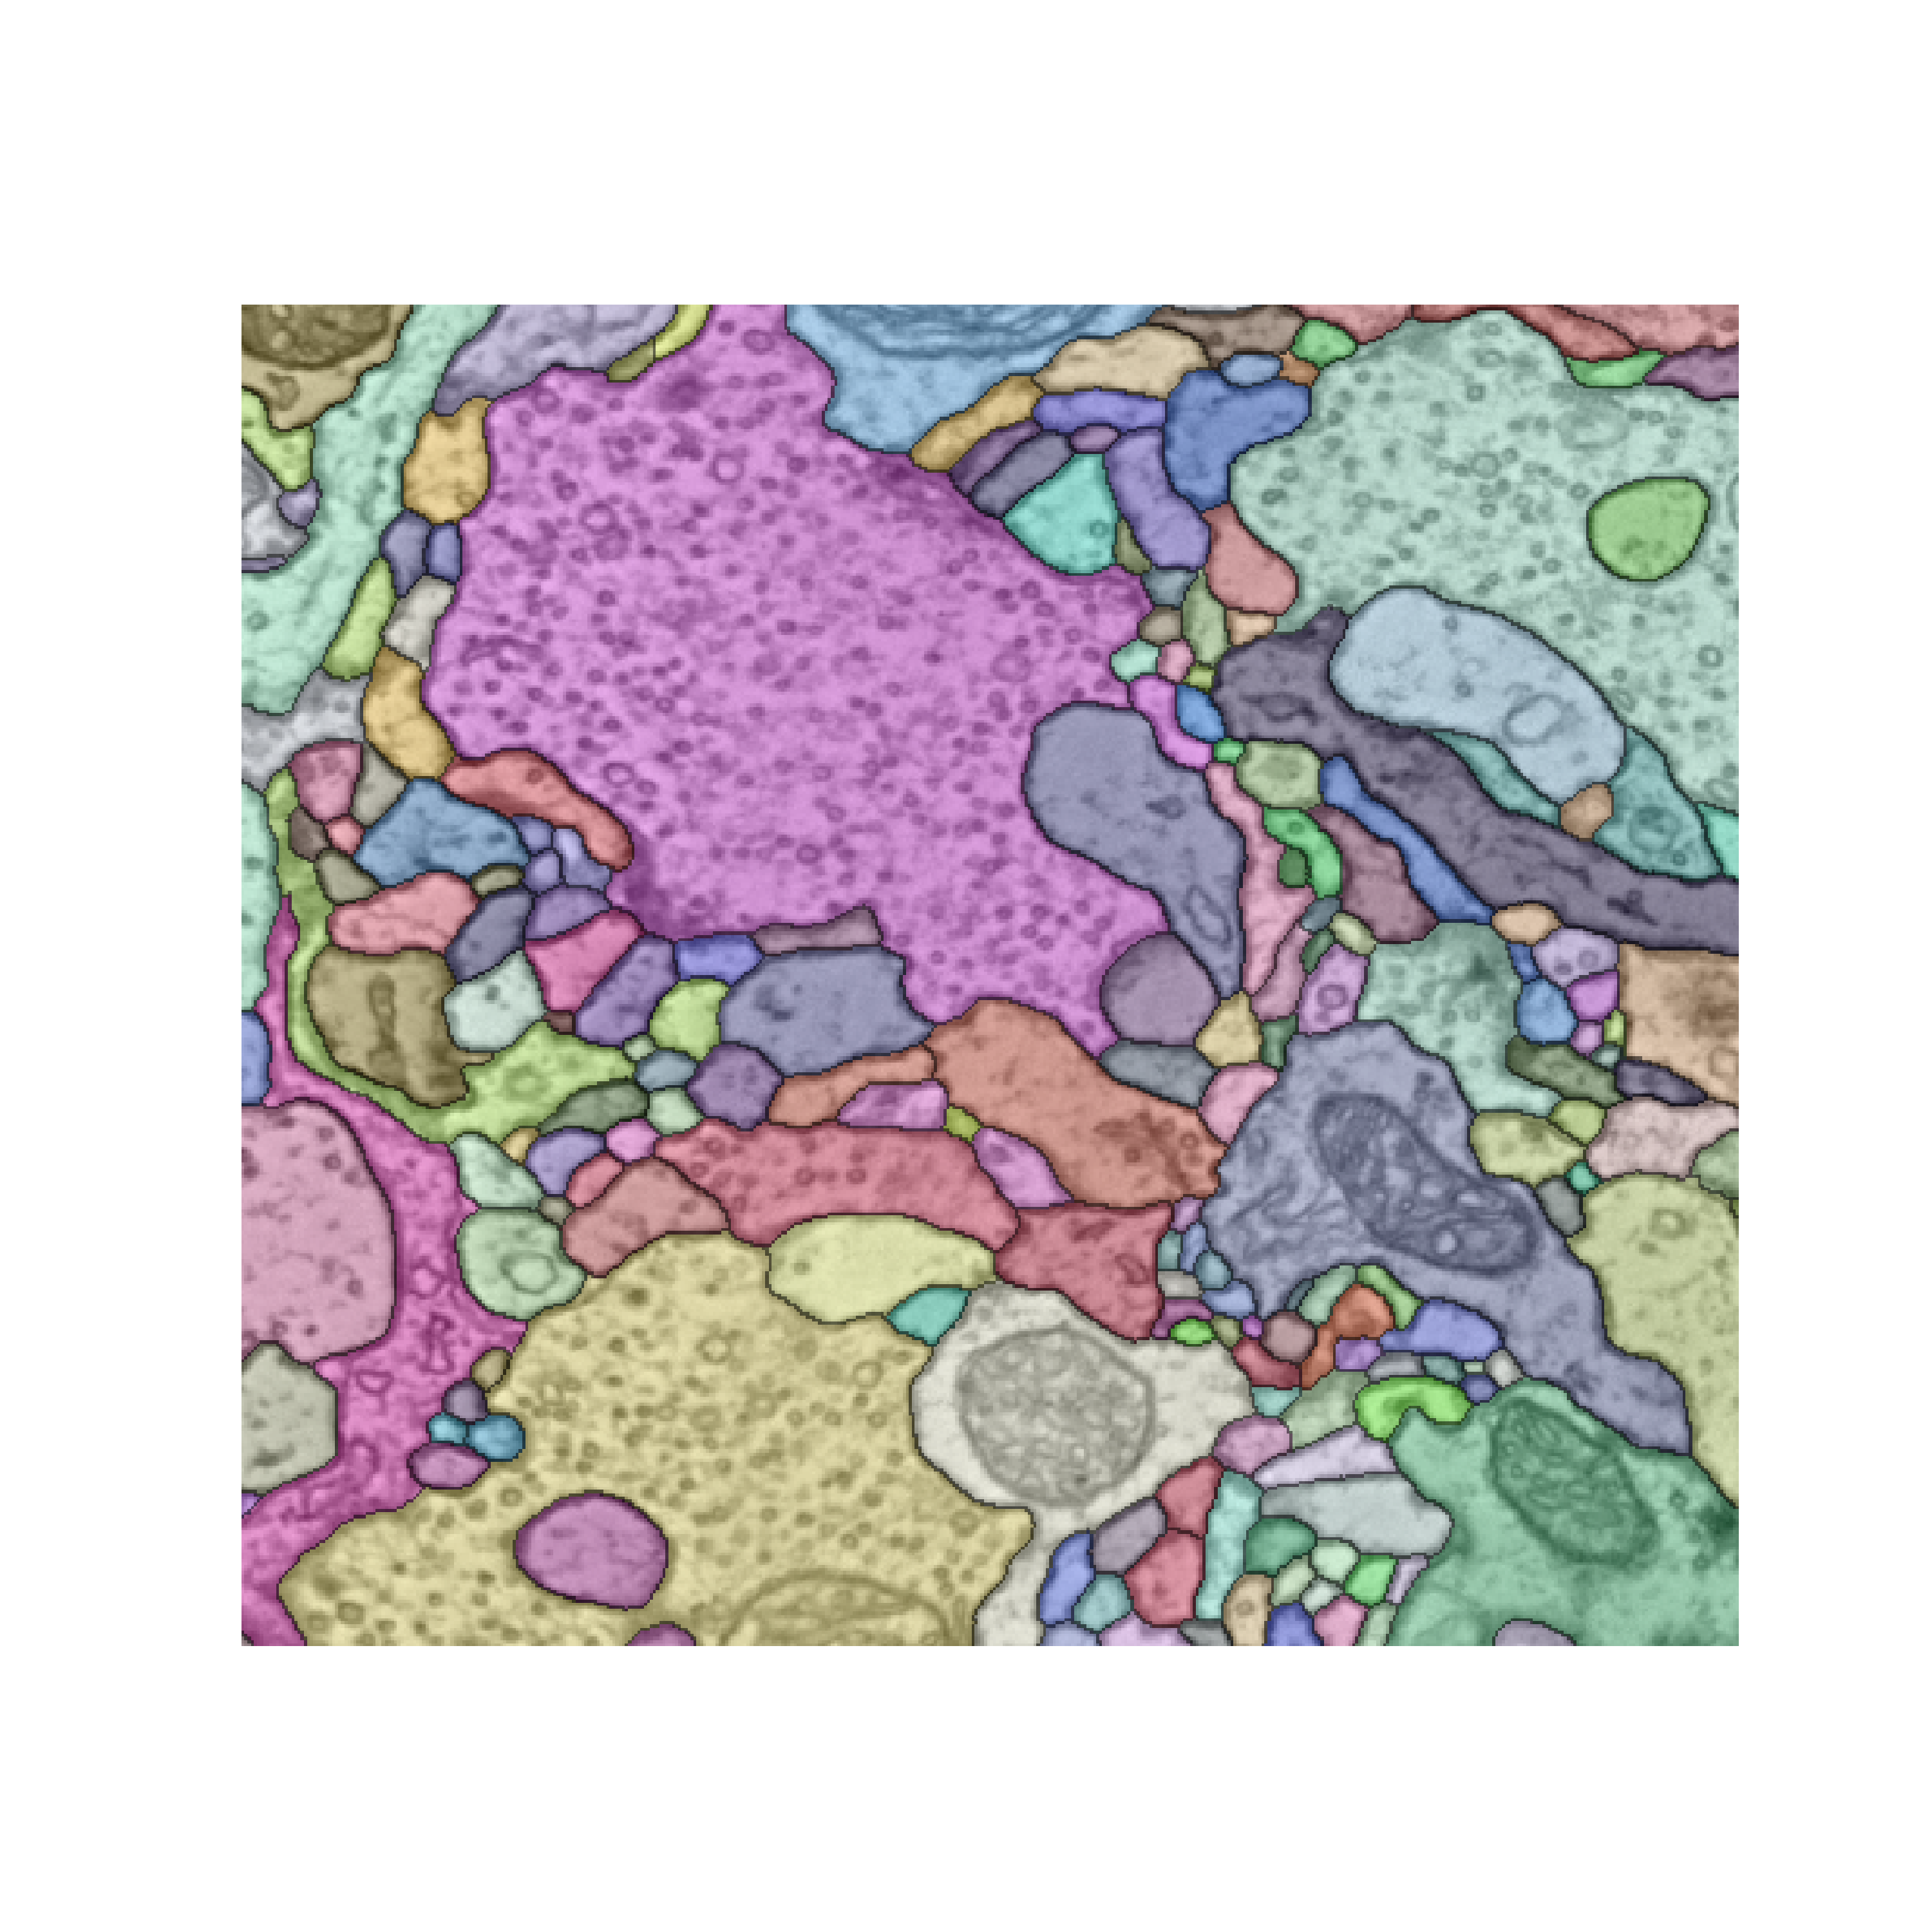
\includegraphics[width=\textwidth,trim=1.80in 1.4in 1.8in 1.50in,clip]{./figs/MWS_segm.pdf} % 0.45
        \caption{Raw data from the validation set overlaid with the final instance segmentation obtained with our method: affinities are computed by averaging overlapping masks (MaskAggr); the final segmentation is achieved by running the Mutex Watershed algorithm on the obtained graph with positive and negative edge weights. Note that the data is 3D, hence the same color could be assigned to parts of segments that appear disconnected in 2D.}
    \label{fig:MWS_segm}
\end{figure}




\begin{figure}[t]
\centering
        % \includegraphics[width=0.4\textwidth,trim=0.25in 0.25in 0.68in 0.36in,clip]{./figs/SSBM_experiments.pdf} % 0.45
        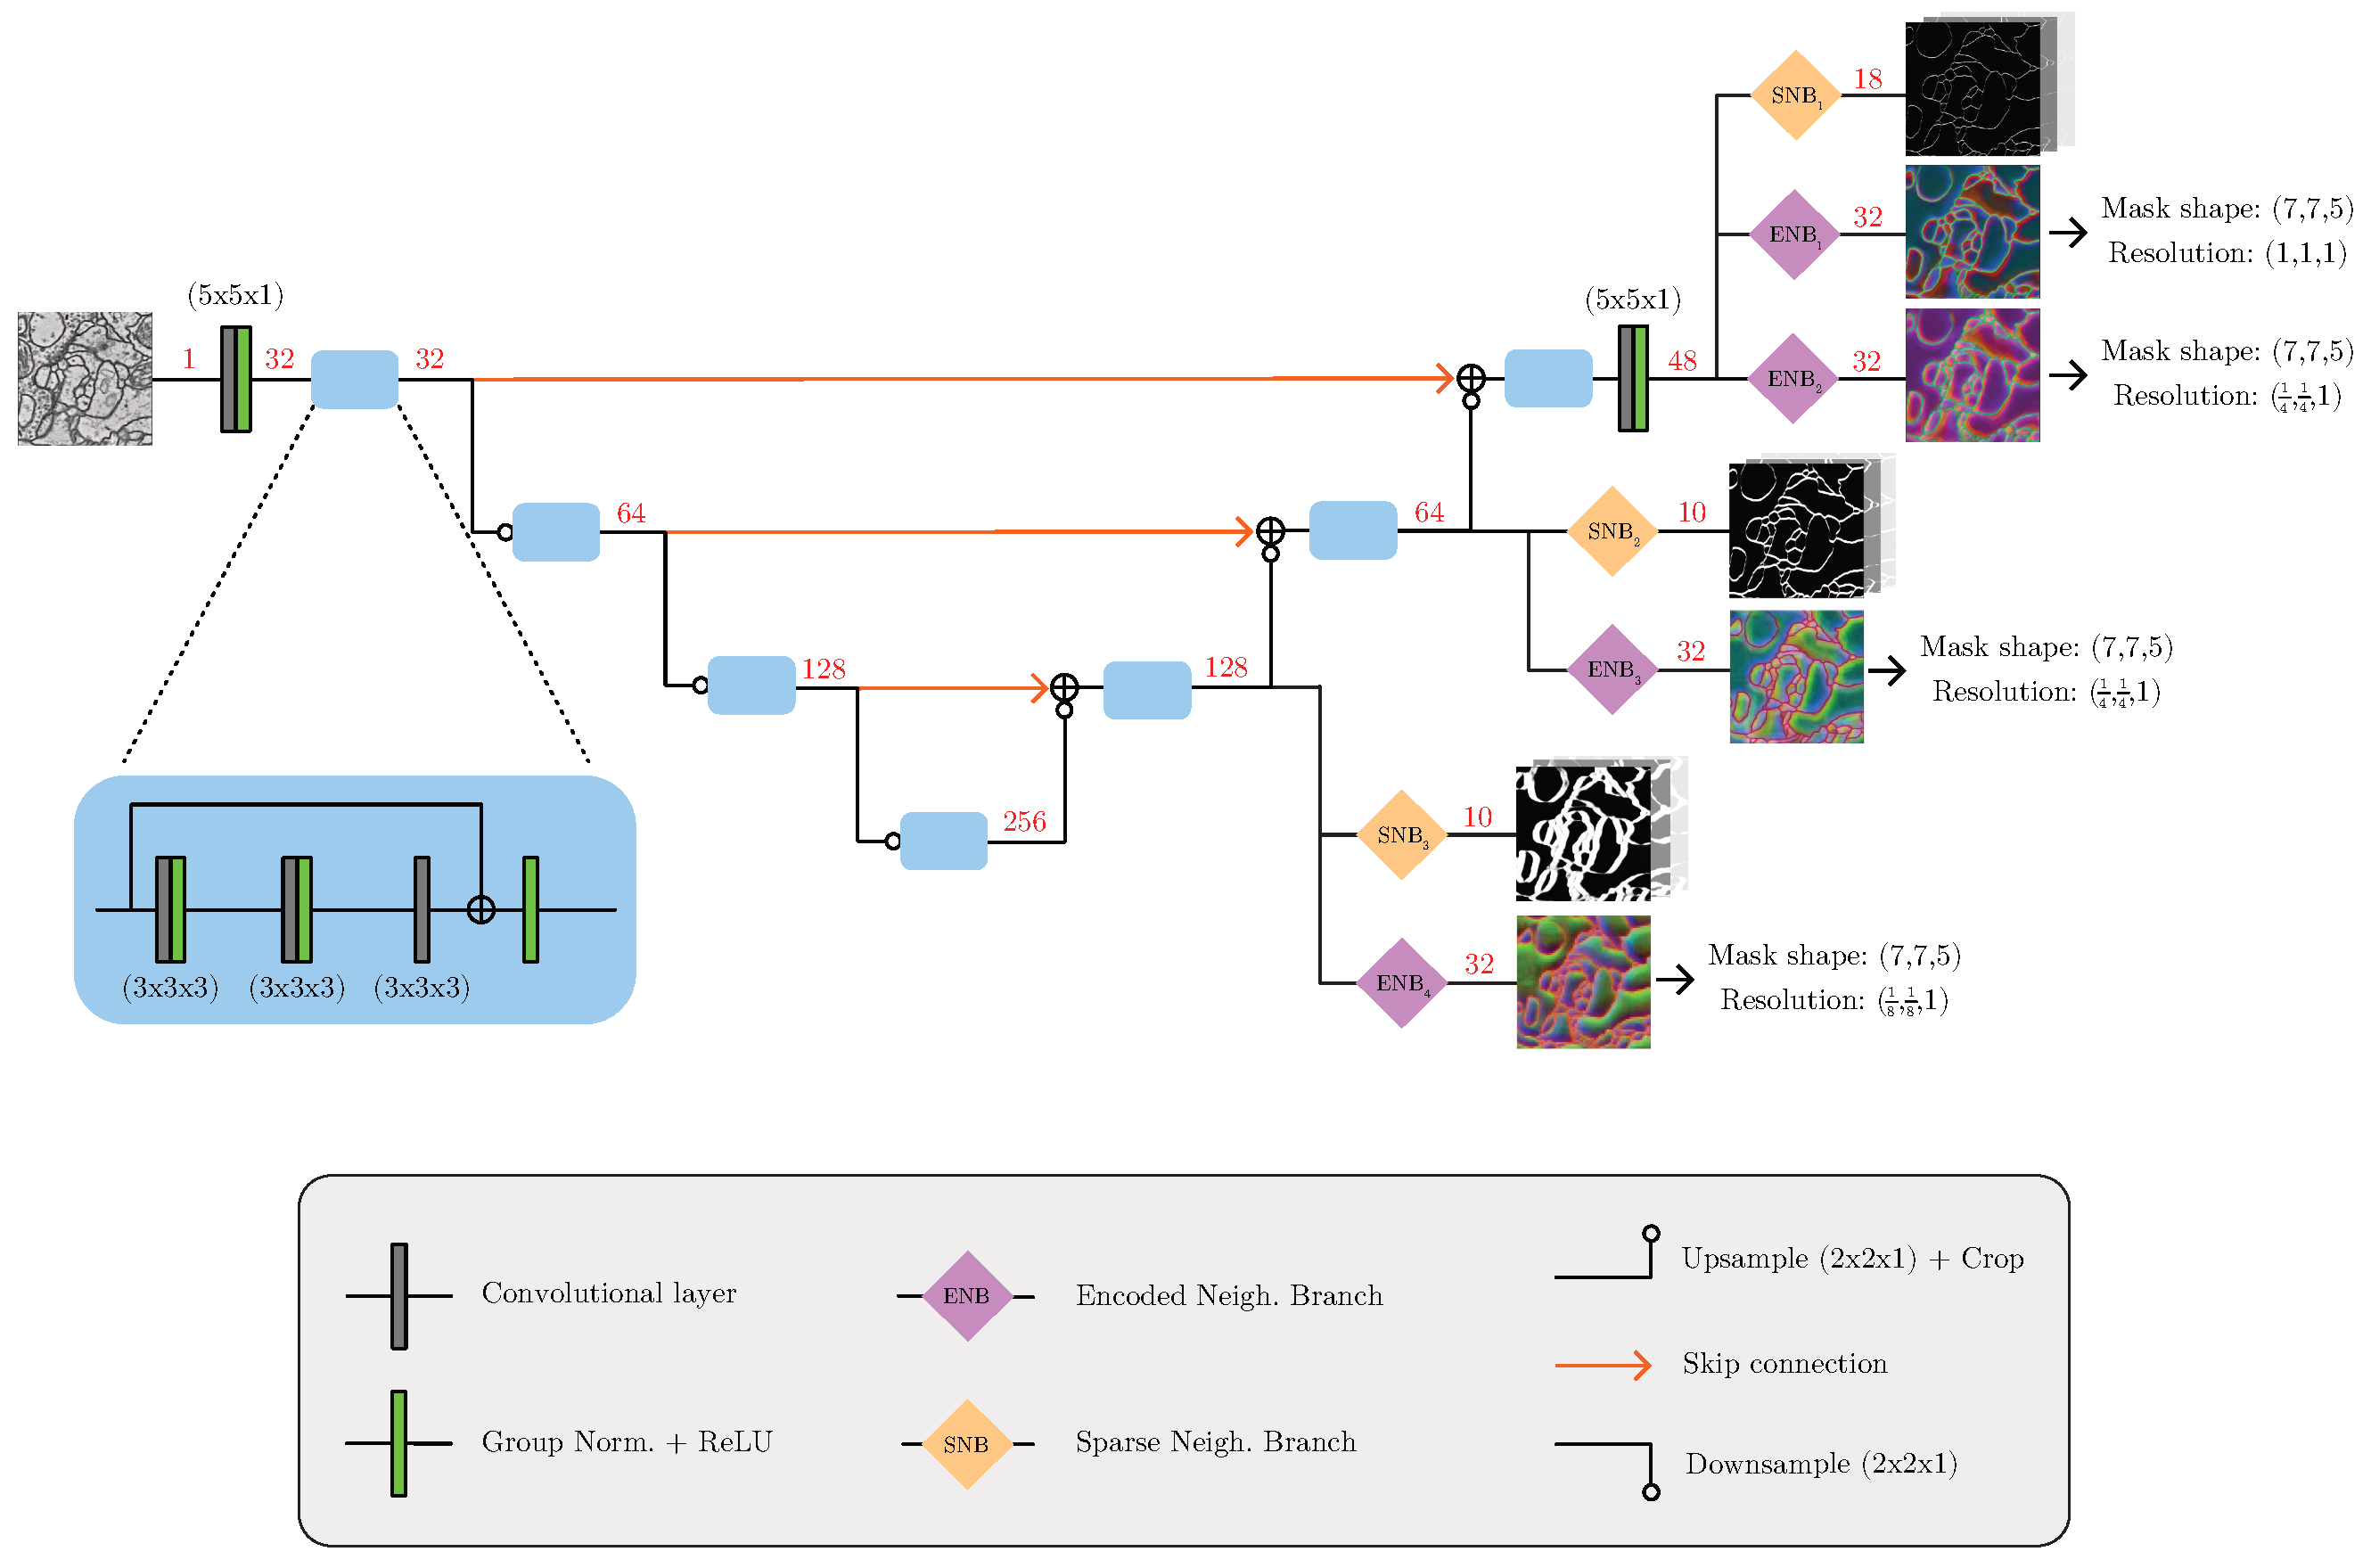
\includegraphics[width=\textwidth]{./figs/UNet_architecture.pdf} % 0.45
        \vspace{1em}
        \caption{\textbf{The architecture of the model}, which is strongly inspired by the 3D-UNet models proposed in \cite{lee2017superhuman,funke2018large}. 
        Red numbers indicate the number of used feature maps.
        As we explain in Sec. \ref{sec:models_details}, in this work we consider three models: i) a baseline model based on the three \emph{\sparseBr branches} SNB$_{i=1,2,3}$, shown in the figure; ii) another model based on the four \emph{\encBr branches} ENB$_{i=1,2,3,4}$; iii) and, finally, a combined model trained with all seven branches shown in the Figure.
        Even though the input of the model is a 3D volume, here, for simplicity, we show an example of 2D input image taken from the stack. As output of the \emph{\sparseBr branches} SNB$_{i=1,2,3}$, we show few channels representing some of the predicted affinities (see Table \ref{tab:neighborhood_structures} for details on the sparse neighborhood structures predicted by each branch SNB$_{i=1,2,3}$). We also show the first three principal components of the encoded masks predicted by the \emph{\encBr branches} ENB$_{i=1,2,3,4}$. All branches ENB$_{i=1,2,3,4}$ predict \maskname masks of the same window size $7 \times 7 \times 5$, but at different resolutions.}
    \label{fig:model_architecture}
\end{figure}

\begin{figure}[t]
\centering
        % \includegraphics[width=0.4\textwidth,trim=0.25in 0.25in 0.68in 0.36in,clip]{./figs/SSBM_experiments.pdf} % 0.45
        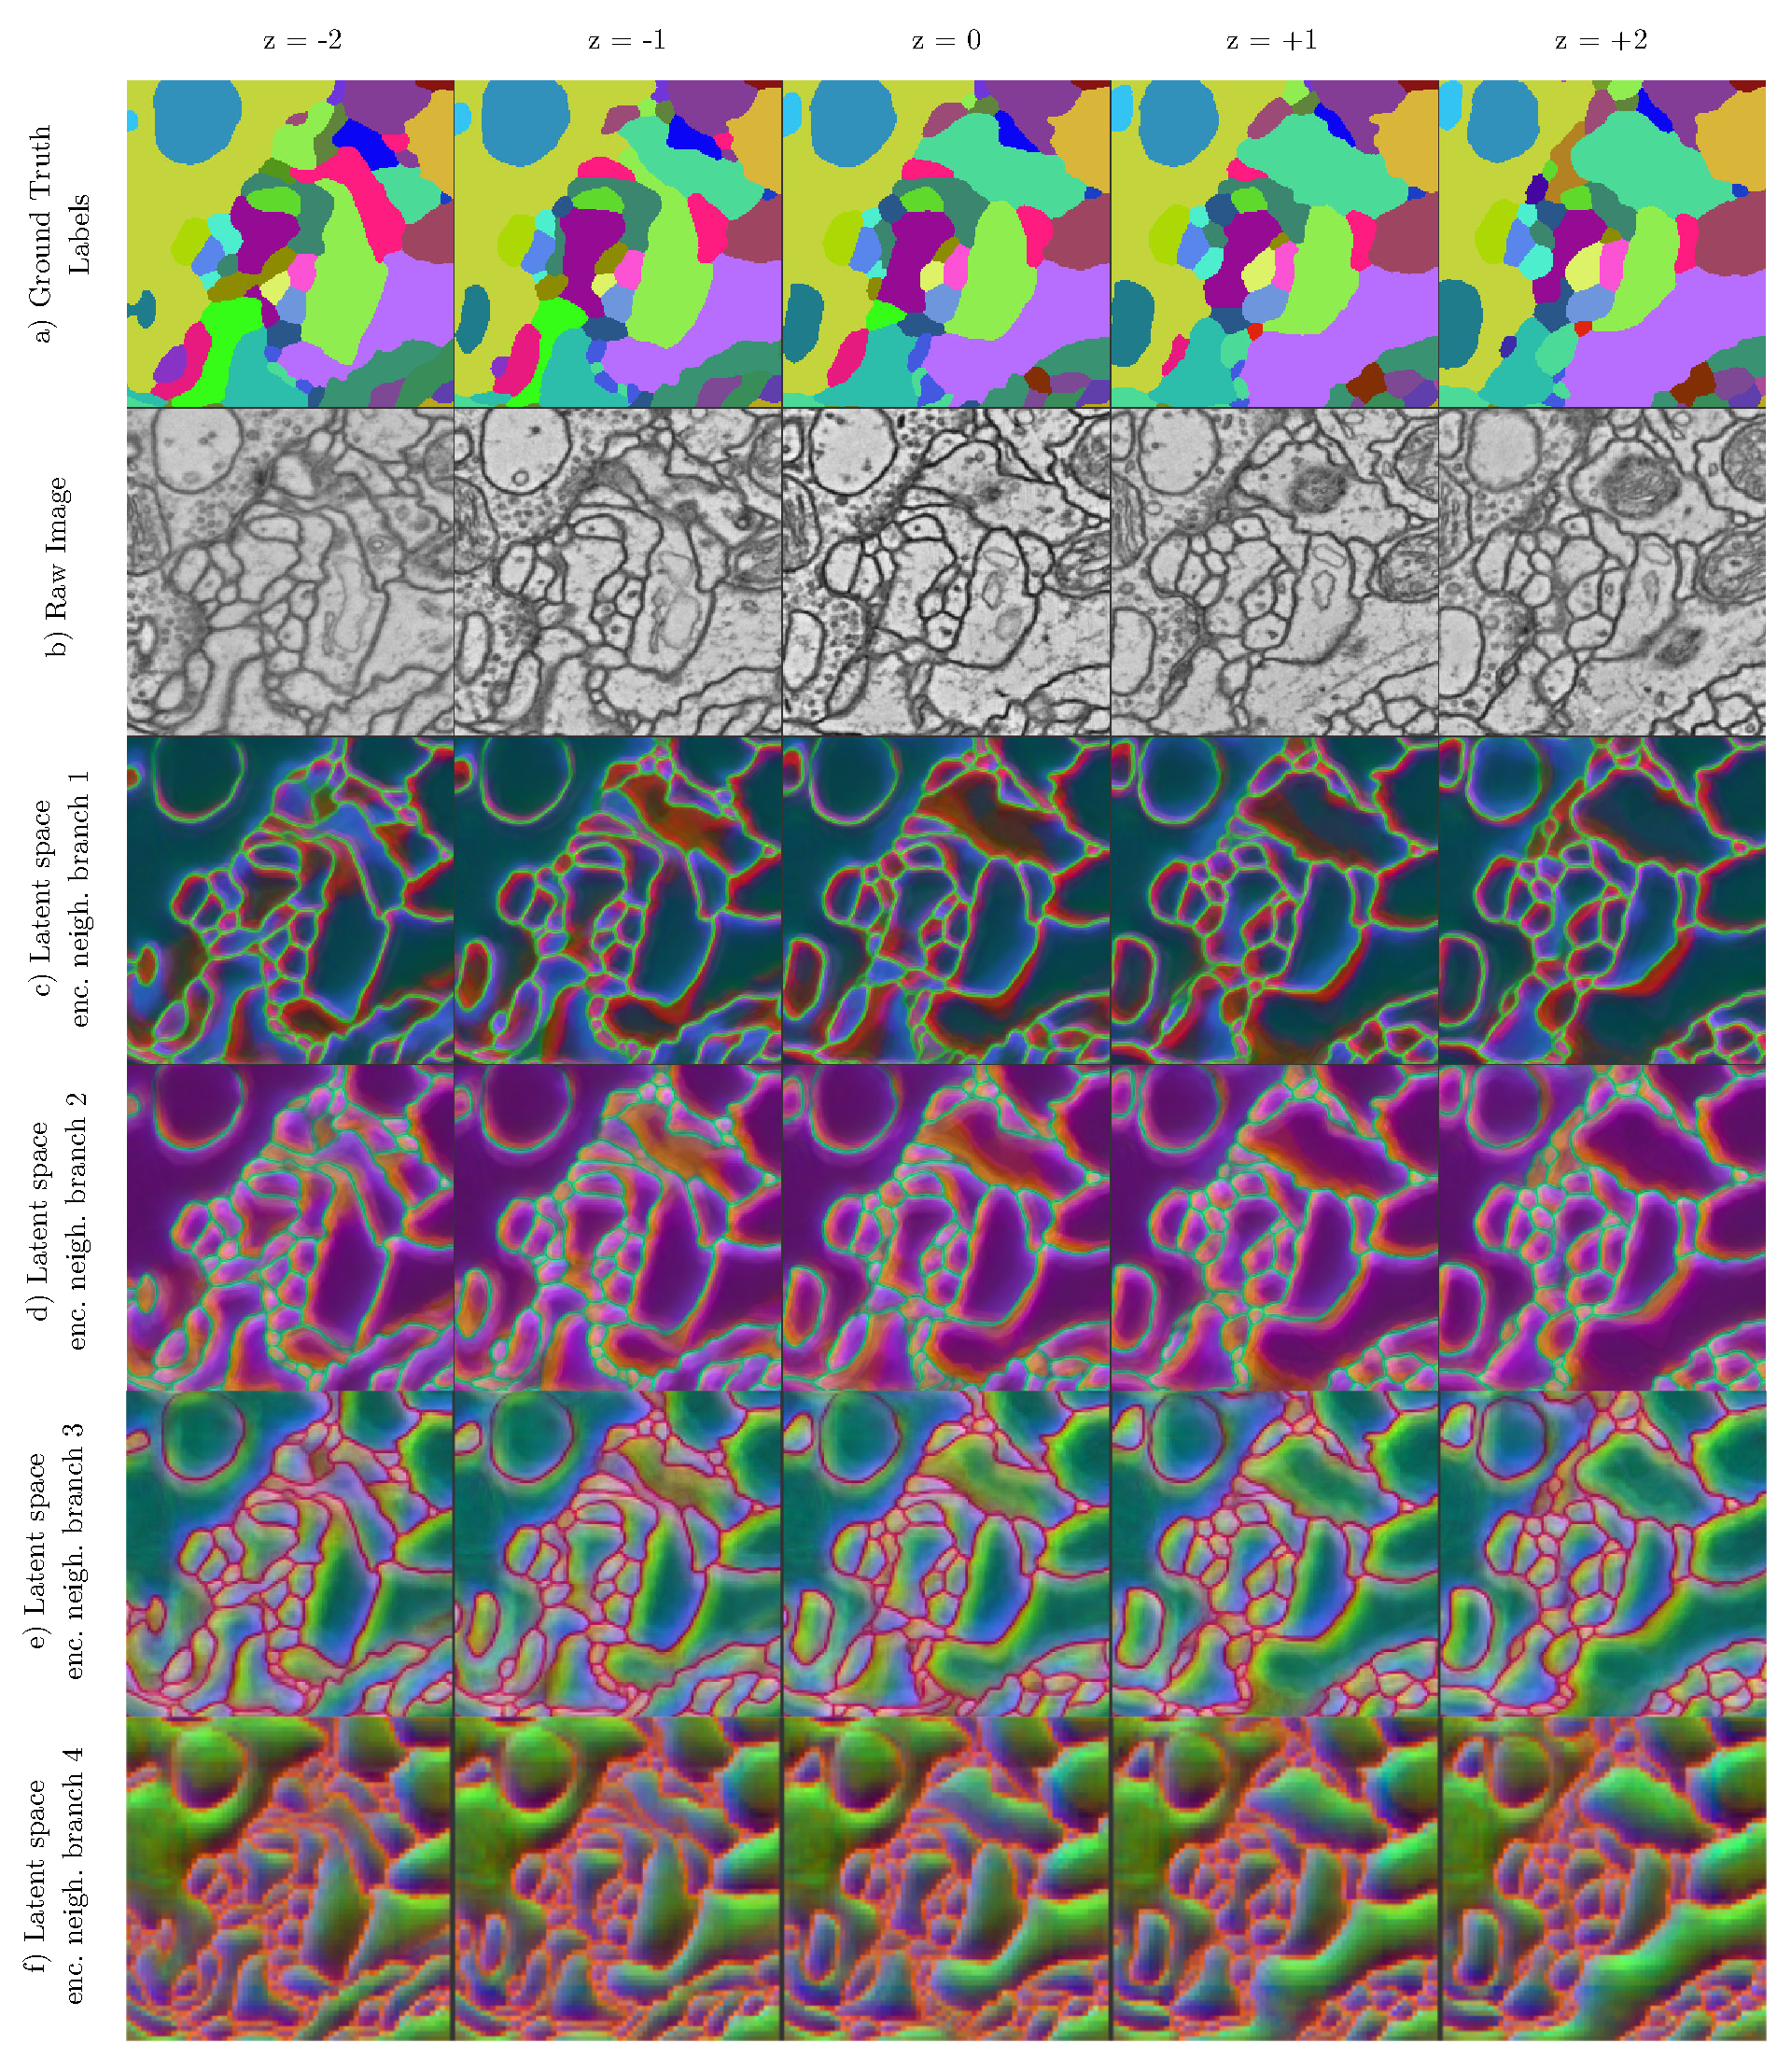
\includegraphics[width=\textwidth]{./figs/PCA_embeddings.pdf} % 0.45
        \vspace{1em}
        \caption{\textbf{Visualization of the predicted single-instance mask latent spaces} -- Each column represents a 2D image from the 3D stack (only five are shown here). \textbf{(a)} Ground-truth labels. \textbf{(b)} Raw image given as input to the model. \textbf{(c-d-e-f)} Visualization of the first three principal components of the $32$-dimensional mask latent spaces predicted by the \encBr branches ENB$_{i=1,2,3,4}$ in our model. Note how latent spaces learned at different levels of the U-Net pyramid show different feature-scales, because they encode \maskname masks at different resolutions.}
    \label{fig:PCA_embeddings}
\end{figure}

\begin{table}[t]
\small
\centering
  % {\renewcommand{\arraystretch}{1.3}
  % \resizebox{\textwidth}{!}{
        \begin{tabular}[t]{M{10em} M{8em} M{8em} M{8em} }
         % Method & \makecell{CREMI-Score \\(lower is better)} \\ \midrule 
\thead{Graph neighborhood\\structure\\(16 neighbors)} & \thead{SNB$_1$\\(18 neighbors)} &  \thead{SNB$_2$\\(10 neighbors)}  & \thead{SNB$_3$\\(10 neighbors)} \\ \toprule 
(0, 0, -1)      & (0, 0, -1)    & (0, 0, -1)    & (0, 0, -1) \\
(-1, 0, 0)      & (-1, 0, 0)    & (-4, 0, 0)    & (-4, 0, 0) \\
(0, -1, 0)     & (0, -1, 0)     & (0, -4, 0)    & (0, -4, 0) \\
(-4, 0, 0)     & (-4, 0, 0)     & (0, 0, -2)    & (0, 0, -2) \\
(0, -4, 0)     & (0, -4, 0)     & (0, 0, -3)    & (0, 0, -3) \\
(-4, -4, 0)    & (-4, -4, 0)    & (0, 0, -4)    & (0, 0, -4) \\
(4, -4, 0)     & (4, -4, 0)     & (-14, 0, 0)   & (-12, 0, 0) \\
(-4, 0, -1)     & (-4, 0, -1)   & (0, -14, 0)   & (0, -12, 0) \\
(0, -4, -1)     & (0, -4, -1)   & (-14, -14, 0) & (-12, -12, 0) \\
(-4, -4, -1)    & (-4, -4, -1)  & (14, -14, 0)  & (12, -12, 0) \\
(4, -4, -1)     & (4, -4, -1)   &  - & - \\
(0, 0, -2)      & (0, 0, -2)    & - & - \\
(-8, -8, 0)    & (0, 0, -3)     & - & - \\
(8, -8, 0)     & (0, 0, -4)     & - & - \\
(-12, 0, 0)    & (-8, -8, 0)    & - & - \\
(0, -12, 0)    & (8, -8, 0)     & - & - \\
-                & (-12, 0, 0)   & - & - \\
-               & (0, -12, 0)   & - & - \\
        \end{tabular}
        % }
        \vspace{3em}
        \caption{\textbf{Sparse neighborhood structures} --  
        In this table, we represent sparse neighborhood structures (see for example the one shown in Fig. \ref{fig:main_figure}a) as lists of offsets $(\delta_x,\delta_y, \delta_z)$ indicating the relative coordinates of neighboring pixels with respect to the central pixel.
        The first column shows the neighborhood structure of the pixel grid-graph, such that each pixel / node is connected to 16 neighbors. In the following columns, we provide the neighborhood structures predicted by the three \emph{\sparseBr branches} SNB$_i$ used in our model (see architecture in Fig. \ref{fig:model_architecture}).
        These neighborhood structures were inspired by the ones used in \cite{wolf2018mutex,lee2017superhuman} but were adapted to our version of the CREMI data that is downscaled by a factor $(\frac{1}{2},\frac{1}{2},1)$. Note that the offsets provided here are given in the downscaled resolution.} \label{tab:neighborhood_structures}
\end{table}





\end{document}
